%----------------------------------------------------------------------------------------
%	PACKAGES AND OTHER DOCUMENT CONFIGURATIONS
%----------------------------------------------------------------------------------------
% !TeX TS-program = pdflatexmk

\documentclass[a4paper,11pt]{scrreprt}
\usepackage[hscale=0.69,vscale=0.79,heightrounded,includehead]{geometry}
%\pagestyle{headings}
\usepackage{fancyvrb}
\usepackage[usenames,dvipsnames]{xcolor}
\usepackage{soul}
\usepackage{wrapfig}
\usepackage[english]{babel}
\usepackage{graphicx}
\graphicspath{ {../graphics/} }
\usepackage{floatrow}
\usepackage{babel}
\usepackage{csquotes}
\usepackage{caption}
\usepackage{subcaption}
\usepackage{multicol}
\usepackage[labelformat=simple]{subcaption}
\usepackage[T1]{fontenc}
\usepackage{float}
\usepackage[backend=biber]{biblatex}
\addbibresource{references.bib}
\usepackage{epstopdf}
\usepackage{fancyvrb}
\usepackage{hyperref}
\usepackage{listings}
\usepackage{color}
\newcommand{\HRule}{\rule{\linewidth}{0.5mm}}
\definecolor{dkgreen}{rgb}{0,0.6,0}
\definecolor{gray}{rgb}{0.5,0.5,0.5}
\definecolor{mauve}{rgb}{0.58,0,0.82}
\usepackage{amssymb,amsmath}
\usepackage{abstract}
\DeclareMathOperator*{\argmax}{\arg\!\max}

\addtokomafont{chapterprefix}{\raggedleft}
\renewcommand*{\chapterformat}{%
\mbox{\chapappifchapterprefix{\nobreakspace}%
\scalebox{5}{\color{gray}\thechapter\autodot}\enskip}%
}
\captionsetup[figure]{labelfont=it,textfont={it}}
\captionsetup[subfigure]{labelfont=bf,textfont=normalfont,singlelinecheck=off,justification=raggedright,labelformat=simple, labelsep=colon}
\usepackage{newfloat}
\DeclareFloatingEnvironment[
    fileext=los,
    listname=List of Equations,
    name=Equations,
    placement=tbhp,
    within=section,
]{myequations}
%----------------------------------------------------------------------------------------
%	BEGIN & TABLE OF CONTENTS
%----------------------------------------------------------------------------------------
\begin{document}

\title{Realtime Classification Engine}
\subtitle{Msc Intelligent Systems Dissertation}
\author{Andrew Haines\\
	University of Sussex\\
	\texttt{ajh21@sussex.ac.uk}}

\date{\today}
\maketitle

\begin{abstract}
With the invent of processing platforms that allow for cheap, commodity hardware to run horizontally distributed applications at unprecedented scale, never before have we seen such an explosion of data collection and processing. Because of this abundance of processing power and ever cheaper storage costs, there is a growing trend to capture and collect events, limited only by what can be instrumented and regardless of an immediate requirement. These persisted events sit dormant in data centers waiting for their vast coffers to be harvested for valuable insights and application. Many of the algorithms and developments that have arisen out of this have relied on the fact that even though such sporadically collected data is noisy, with enough of it, the law of large numbers suggests that signals can still emerge and be fed into a new breed of intelligent systems\cite{bigdata}. The problem with this approach is that, although tractable to large institutions and organizations, smaller, more modest individuals will not have the infrastructure or financing to support such data collection even though their reach is enough to warrant its need. Tech startups in particular face this problem with a careful balancing of the business insights and user requirements they can provide at a trade off of vast equity deals in seeding rounds.\\

In this project we attempt to design and build a closed domain application that runs at 'big data' scale but on a single machine instance. The closed domain of the application is one of a classifier that, given an entity or event expressed in a feature space, it recommends suggested classes based on a continuous stream of online data input. The ideas and concepts that semantically define this recommender are nothing new but its implementation and structure is novel, excelling previous standards by making extensive use of modern computer architecture to process events far quicker than traditional techniques.

\end{abstract}

\tableofcontents

\chapter{Introduction}
More and more large institutions these days rely on the analysis of vast quantities of data to inform business decisions and provide performance feedback. From tracking the performance of advertising campaigns, constructing weather models, and powering recommendation engines, Big Data processing is rapidly becoming the cornerstone of the online technology industry. Large companies such as Google and IBM spend hundreds of millions of pounds in capex to construct and maintain the processing platforms required to mine this data. These systems are typically generic constructions developed across many thousands of machines and delivered company-wide to cater for all business units in the organization. Resources such as storage and compute time are then shared across all applications of the company. To accommodate this, either fully distributed but virtualised operating systems that coordinate a 'grid' of machines and networking topologies or complex multi processing core workhouse instances are used to execute such data hungry applications. There are many different paradigms and approaches for powering these systems but they all share one common drawback - these infrastructures come at the cost of an astronomical financial footprint, costing several hundreds of thousands of dollars for comparatively modest setups to multi million dollar investment for corporate scale facilities.

The focus of this project is whether the existing designs and ideologies of these approaches can be borrowed, blended and re-devised to create a system with a real life intelligent application that runs at big data scale but with a fraction of the monetary expenditure. If such a system is possible, the value to individuals where existing big data solutions are out of reach could be unprescended.

\chapter{Background}
\section{Big Data Processing Paradigms}
The current state of the art in big data computation falls primarily into three distinct camps.
\subsection{Batch Processing}
The first archetypical model is one that follows a batch processing methodology. The concept is that data is persisted onto a distributed file system in near raw form. Processing then operates on the data either as a one off task for insight analysis or bootstrapping purposes or, at periodic intervals that produce transformed data that can be used in downstream processes. To illustrate this, consider a possible implementation of a 'trending now' feature on a large web property's home page - used to inform users of what is currently popular on the domain at that time. 

To determine this, the web property instruments all interactions with various content on its systems. This could be tweets sent from a mobile device app or news articles clicked on via a user's web browser - all events are logged to a central analytics system with a pre defined payload. This payload could contain information about the user\footnote{gender, age, personal preferences, etc}, the local time the event occurred at, information about the device, the content UUID interacted with... the tuple of data that could be chosen is endless. The analytics servers then typically place the event, via a messaging system onto the distributed file system\footnote{This file system is distributed in the sense that the data actually sits on multiple machines possibly in geo graphically diverse data centers but appear as if it is one contiguous structure of files.} in a '\texttt{rawevents-YYYYMMDDHH-xxxx}' series of files. A scheduled task then runs at say every hour and consumes these latest files, extracts named entities from them and contructs a histogram of their occurrences. The named entities are then ranked according to the histogram's frequency and the top x results are persisted into a '\texttt{trending-now-YYYYMMDDHH}' timestamped file. This comparatively tiny file is then sent to all the client facing webservers and powers the last hour's 'trending now' list.

Using the batch approach enables the data to be processed 'offline' in the sense that data is processed some time after the events have occurred.  This has a number of advantages over the cost of not being real time. Firstly, the programming concepts can be far easy to implement. Consider the calculation of a median value of a vast list of numerical objects. Using batch you would simply sort the list and pick the middle one as you have all the data for that given hour available. Indeed, if you choose to not remove the intermediate '\texttt{'rawevents'} files then larger periods can be scaled up by simply increased the file ranges. Handling in the event of error is also far easier as processing can easily be rerun. The other downside is that the demand on storage capacity is huge but, given the growing trend to capture all data and archive it for later insights, this tends to already be available.\\

There are 2 main concepts within batch processing that allow it to structure the control flow of the application.

\subsubsection{Map Reduce}
This technique is an adaptation of an old functional programming paradigm where by two phases of computation are established - the map phase and the reduce phase. Google took this paradigm and ported it to a distributed setting in 2004\cite{mapreduce}. The general idea is that during the map task, execution is moved to where the data is rather then data being moved to whether the executable code lies. The reason in the big data setting should be obvious as the IO costs involved in transporting vast quantities of data to executor machines is fair costlier and time consuming then moving a small executable to each of the machine that store the event files. Such machines are referred to as data nodes. Execution in the map phase then runs on the data nodes and is used to filter, transform and assign special keys to each record that this data node holds. The output, being typically alot smaller, 'shuffled' to reducer nodes which may (some IO costs) or may not (no costs incurred) be on different machines before finally being sorted by the special keys assigned during mapping. This allows all items assigned to a particular key to be available on a single reducer. In the case of the trending now example, this would equate to each instance of a named entity being sent to a single reducer so that it's component of the histogram - its particular count - can be computed (see Figure \ref{fig:MapReduceEx}). In 2011 Yahoo open sourced the HadoopMR\autocite{hadoopMR} module that forms part of the hadoop operating system.\\

\begin{figure}[h]
\centering
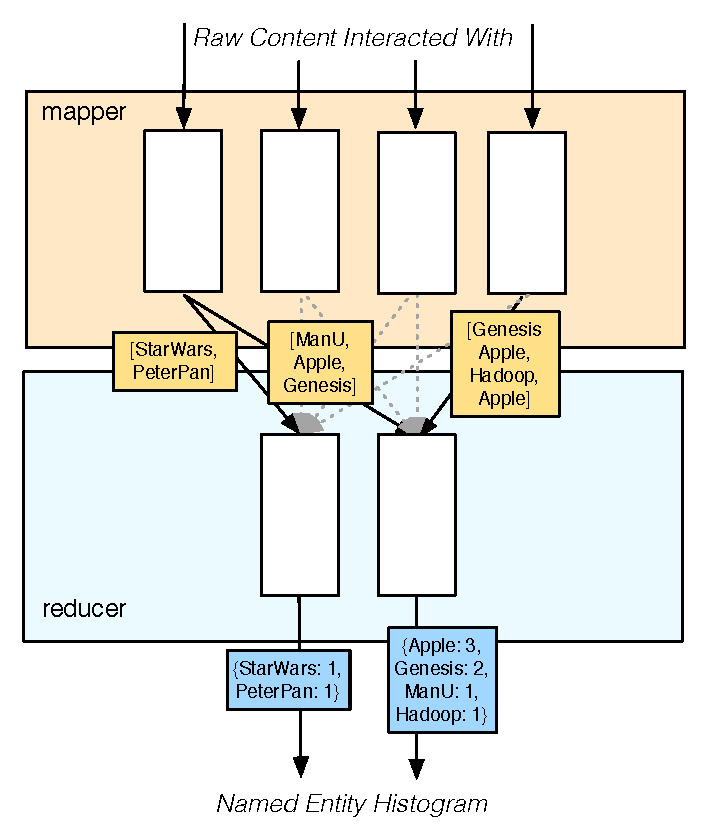
\includegraphics[scale=0.7] {MapReduceEx.pdf}
\caption{MapReduce Trending Now Example. For Brevity only output from 2 mappers are shown. The inputs to the process are the raw content data and the mappers determine which named entities are present. These are then keyed on the textual representation of the entity and all entities of the same name are sent to a single reducer. The output is then a frequency count of all named entities}
\label{fig:MapReduceEx}
\end{figure}

The problem with this approach is that, although it scales well when the distribution of the keys is uniform, in the face of skew in the key set, this bias is propaged down to the reducer load and can mean that a small number of machines can do the majority of the work. Also, as we have seen from the trending now example, the calculation of the distribution of terms is only one part of the entire process. It was assumed here that the entities of all the content that was interacted with had been previously computed. To do this using Map Reduce we would need another set of MR tasks that would extract the content from the raw events, normally only defined by the UUID, prior to the task described. The output is also just the raw counts, we would need a further step to then sort the entities by their counts and only persist the top x. This illustrates what typically happens with complicated MR applications in that a number of sub tasks of mapping and reducing have to occur with intermediate temporary files coordinating the data flow between them. This can be both limiting in how a application is structured and also inefficient due to unnecessary persistence of these temporary files. To solve this the DAG approach was devised:

\subsubsection{DAG}

\begin{figure}[H]
\centering
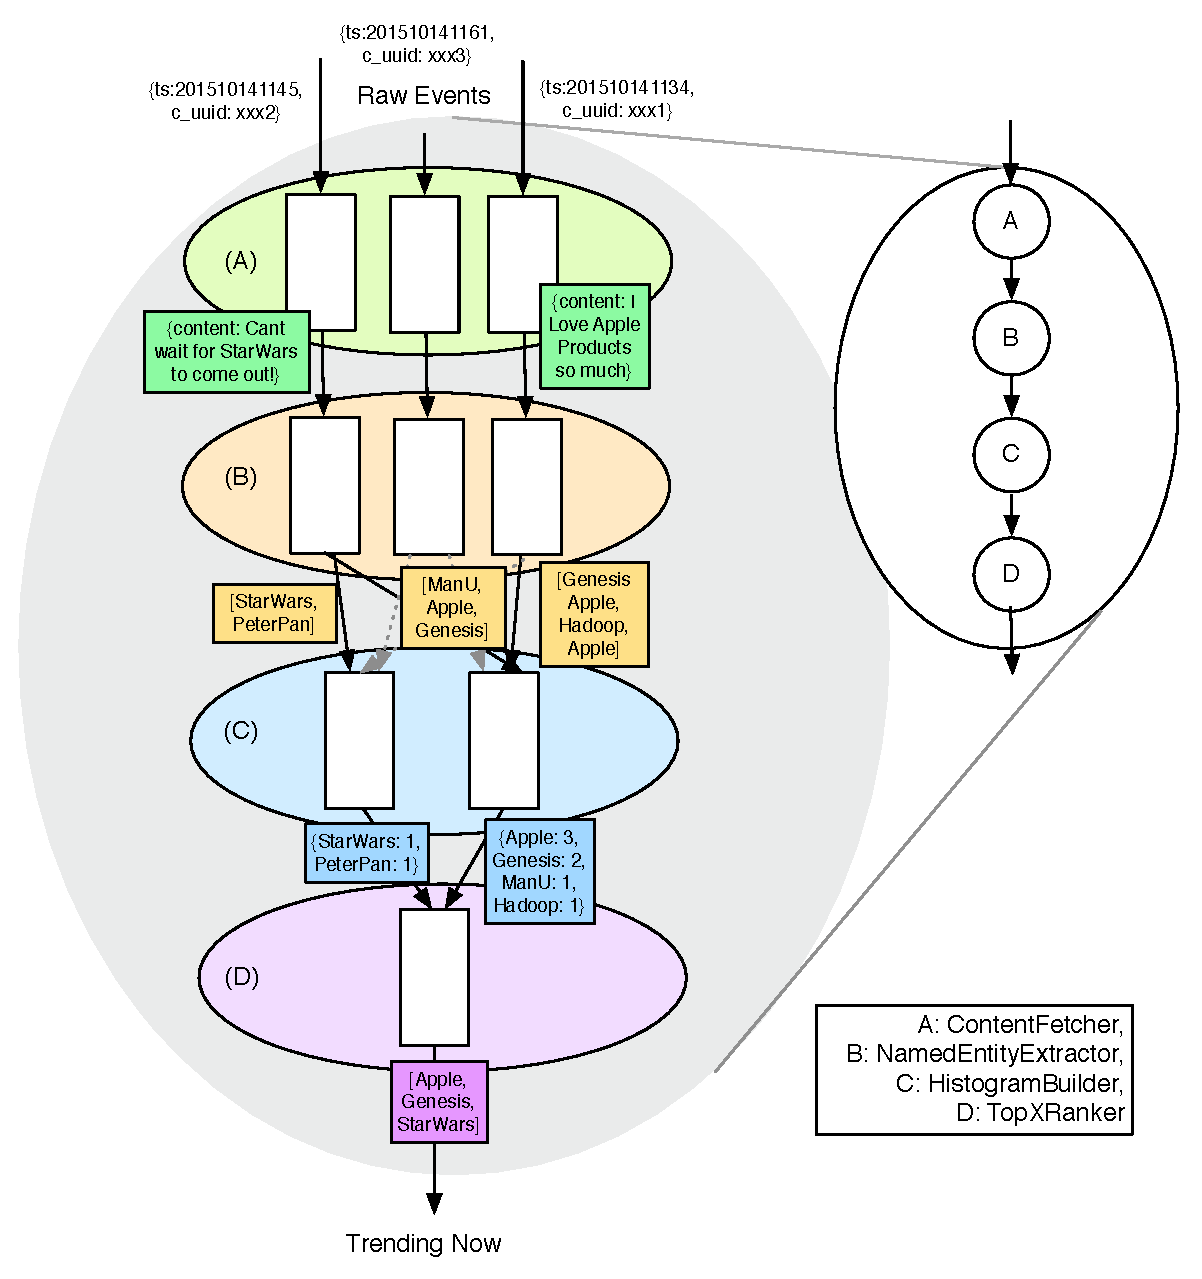
\includegraphics[scale=0.65] {DAG.pdf}
\caption{DAG Trending Now Example. In this example the entire application is shown, not just the histogram building. Data flows through the graph along the edges to the nodes. In this example, the DAG framework is able to determine that both the content fetcher and the name entity extractor need never move any data around and so the computation actually happens on the same nodes without ever having to write to disk}
\label{fig:DAGEx}
\end{figure}

The Directed Acyclic Graph\cite{dryad, spark-paper} approach tackles the deficiencies of MR by defining a graph of tasks that have to be executed concurrently. Nodes in the graph are sub tasks that need to be performed and the edges are data flows between them. Nodes are distributed as in MR by moving them to where the data is but there exists far more flexibility in how an execution flow can be maintained and structured. In the trending now example, a node can exist for extracting the entities of the file, where the determined entities are then fed into the distribution calculation node to obtain counts prior to another node that then filters out the x largest entities (see Figure \ref{fig:DAGEx}). Libraries such as tez\cite{tez-site} and spark\cite{spark-site} are two popular frameworks currently gaining traction in the industry.

\subsection{Stream processing}
One of the big problems with batch processing is that it is not real time. For most applications this isn't too much of a draw back but imagine budget caps on an advertiser spend. Waiting for the next hour's processing window to cut off an advertisers supply could be extremely costly. Assuming that processing never overruns\footnote{There is overhead with starting up distributed tasks that can easily make stall resource allocation and cause SLA's to be missed}, near realtime updates could be possible by reducing the processing window of the batch to a few minutes to help mitigate this issue but this isn't going to help a nuclear cooling processor from reacting to a sudden over heating. Stream processing provides a solution to this by processing events in a stream manner as they enter the system and distributed across a cluster of nodes. This means that events are processed, for the most part, either directly from the network bus or in a temporarily buffer, but never needing to be saved on the distributed file system. Processing is structured as a topology using concepts such as spouts and bolts to represent the data flow and processing respectively. In the trending now example, processing occurs in a very similar manner to that of the DAG approach. The difference being of course that at no point does a node get to see anything other than the current event. This is fine in our trending now example until we get to the ranking stage. \\

Choices have to be made in streaming about concepts like where an accumulating histogram is stored and for how long does it persist for? There is no point in keeping the histogram for all time as this defeats the purpose of the trending \textbf{\textit{\underline{now}}}. One option would be to reset every hour, assuming the behavior of the batch processing methodology - except that it wouldn't. A few seconds after the reset and there may not be enough data seen in the histogram to make accurate predictions meaning that periods just after each reset are inherently noisy as the law of large numbers does not hold. Another approach would be a rolling window but this means that you need to keep all events in memory for each window. The larger the window the more likely to exhaust memory whilst smaller windows may not capture enough data. Also consider the median calculation mentioned previously. Without access to all the events, online versions such as a TDigest\cite{tdigest} need to be used which are far harder to implement and understand. Not only is stream based programming a lot harder but they are also extremely sensitive to the throughput coming and what can actually be processed. If your cluster is not large enough to process the influx of events coming into the system, then events are either dropped or buffered, hindering it's real time nature.\\

Obviously the upside of the stream approach, other than it's realtime operating behavior, is that it's also super fast as IO is reduced to bare minimum. Apache Storm\cite{storm-site}\footnote{a commonly used distributed stream processing framework open sourced from Twitter\cite{storm-twitter}. Apache Spark also offers a streaming mode but underneath the hood this is really a micro batch mode to approximate real time\cite{spark-streaming-paper}} claims to be able to process 1M events a second using just a 10 node cluster\footnote{It is worth mentioning that the author's experience of such throughput requires slightly more nodes in a real setting}. Furthermore, if storage capacity is deemed a premium, then this approach can allow big data processing to function without the need of a distributed file system. 

\subsection{Vertically Scaled Systems}
On the other side of the technology spectrum, high throughput processing used in real time exchanges such as those within financial and scientific industries, are able to process huge streams of data but instead of scaling horizontally by adding more machines into a cluster, a single workhouse instance is used with multiple CPUs, huge memory addresses and dedicated transport buses that coordinate the data between. These are concurrent systems that are considered to scale vertically because obtaining more processing power and memory involves the reconfiguration of the instance itself by adding better CPU's or memory modules. These bespoke systems execute code that is specifically tailored to the underlying hardware which makes them incredibly efficient and able to outperform similar speced Hadoop or Storm clusters. Although typically favoring CPU bound tasks, these so called 'supercomputers' can still process vast amounts of data.

At the same time, certain applications that utilise processing of large matrix operations can be performed on GPU processors at speeds far exceeding standard CPU's due to complex instruction sets and dedicated core and transistor architectures customised for graphic processing. Spatial models such as KMeans and CF algorithms can be structured to make the use of these chipsets and perform the computational aspects of learning and prediction in a fraction of the time it would take on a traditional CPU. BidMach\cite{bidmach} is a GPU directed machine learning library that is quoted as being able to cluster the MNIST image dataset into digit clusters on a single Titan-X GPU equipped system in only twice the time of a 128 core cluster\cite{bidmachbench}. Although impressive, this library is only really applicable to certain applications that can be formed using matrix representations where there is a large CPU bound overhead. It still suffers from the plight of processing large volumes of data if the application is IO bound.

\begin{figure}[h!]

\centering
\caption{An example of a 2 core event driven data flow using disruptors to coordinate the transfer of events}
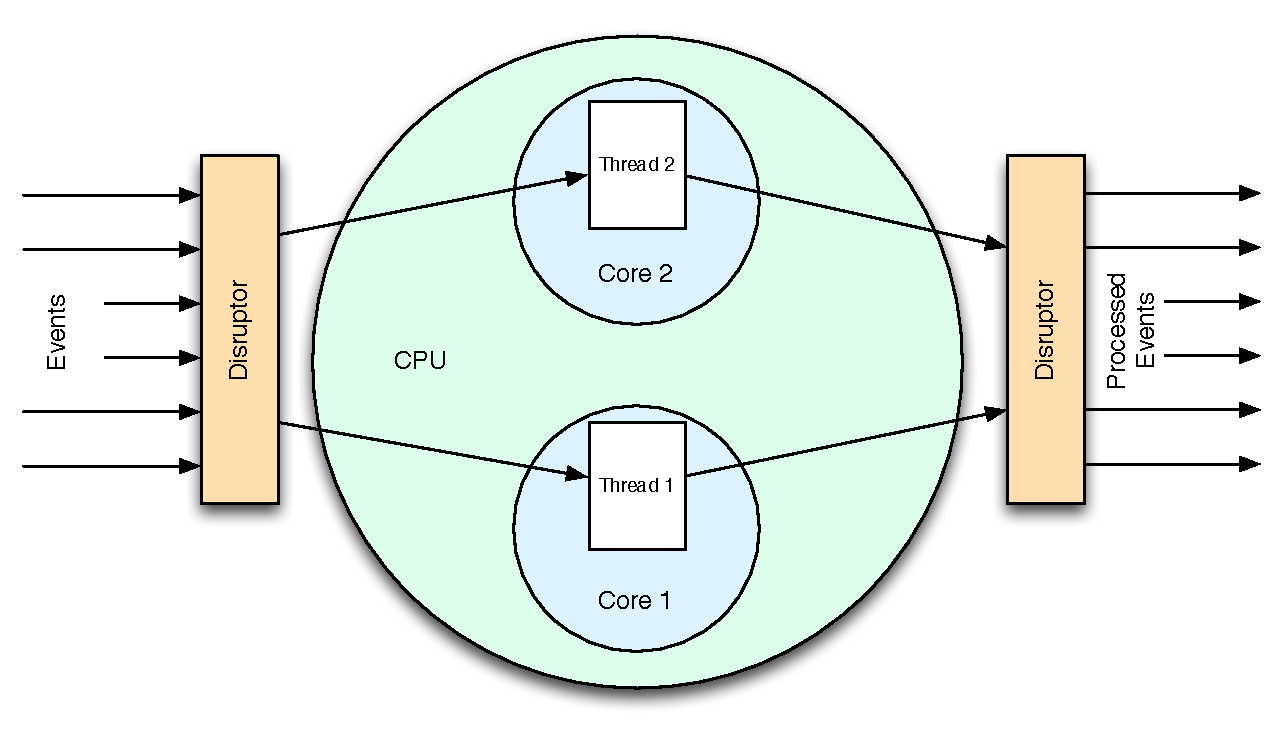
\includegraphics[scale=0.65] {disruptor-ex.pdf}
\label{fig:disruptor-ex}
\end{figure}

Further to this, the LMAX exchange in 2011 released a high throughput processing toolkit that borrowed from similar principles of software and hardware cooperation. Using techniques borrowed from synergising hardware and software, this toolkit is capable of supporting 25M events a second on a single commodity instance\cite{disruptor-paper}. This is not actual computational work mind, just moving events from one conceptual area of a program to another under concurrently safe conditions. None-the-less, achieving such high rates of transfer in in a thread safe manner is still highly impressive. It accomplishes this by using lock-less queues known as \textit{disruptors} that exploit a perfect \textit{mechanical sympathy} between high level programming paradigms and the under lying hardware infrastructure. The basic idea is that disruptors can act as brokers for events, passing them to different areas of code that may or may not be on different threads. This enables event driven design where threads are only used to pin execution to a particular CPU core\cite{processor-affinity}. These long running threads then can operate on the events from the disruptor using the single writer paradigm which ensures that write contention is no longer a concern and only care about visibility to other reader threads need be considered(see \ref{fig:disruptor-ex}). The worker threads can then pass events through the system without costly synchronisation and thread context switching.

Disruptors obtain their ultra fast design by utilising cache line structures and memory barriers present on modern cpus. They are essentially queues implemented in ring buffers where the majority of access is completely unsynchronised - care only be taken to ensure that threads have visibility of events on the buffer. Using a \texttt{volatile} pointer to the index of the buffer, as long as all event processors do not read past the writer position, no locking is required. 
\floatsetup[figure]{capposition=beside,capbesideposition={top,right}}
\begin{figure}[h]
\centering
\caption{The ring buffer at the heart of the disruptor design. For clarity the writer and reader positions are illustrated as if they are concerns of the Producer and EventProcessor respectively - however this is not the case in implementation as the ring buffer owns the pointers in order to ensure \(writerPos < readerPos\)}
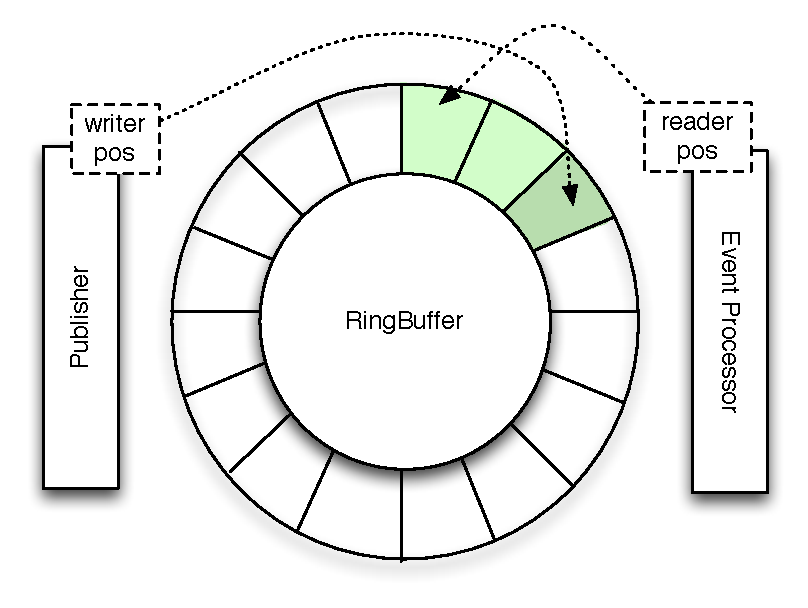
\includegraphics[scale=0.65, trim=0 10 0 0, clip=true] {ringbuffer.pdf}
\label{fig:ringbuffer}
\end{figure}

In the one scenario where the reader and writer are pointing to the same index, CAS operations are used to \textit{busy wait} on mutual exclusivity on this pointer but without coordination amoungst many threads. Under low contention, CAS operations are extremely efficient. Furthermore, as long as the invariant of \(writerPos > readPos\) is held, unlike other cyclic buffers, no end pointer is needed as data can be overwritten when the buffer wraps around.

\section{Machine Learning Applications at scale}
One of the major fields to utilise such large quantities of data is Machine Learning. Tasked with finding systematic patterns in the data and providing classifications and recommendations, ML techniques are used throughout large tech companies to enrich the user experience and provide business analytics. So much so that further abstractions have been provided on top of the data processing paradigms already discussed to enable quick implementations of standardised algorithms and techniques. Libraries such as Mahout\cite{mahout-site} run on top of the hadoop platform and provide scalable interfaces to Logistic Regressors, Random Forests, Collaborative Filtering, etc that engineers can use out of the box at scale. All they need do is chose an algorithm, direct it to the data they wish to be analysed with appropriate hyper parameters and the framework does the rest. Spark in fact is so popular with machine learners that it has bundled its MLlib library as part of the core kernel of the framework, focusing on ML at it's heart. When we move into the streaming implementations as provided by Spark's MLlib library for example, the same considerations mentioned earlier need to be applied in the development of how data is structured and processed at each stage of the computation.\\

Similarly, the popular scientific computing package MatLab offers parallel computing support via its Distributed Computing Toolbox that can utilise 64 CPU cores and beyond, exposing ML libraries to vertically scaled options.

\chapter{Motivation \& Scope}
As seen, there exists a plethora of frameworks and libraries that enable large machine learning applications to be developed at unprecedented scale. But these approaches all have their draw backs. With typical server instances costing upward of \$5K, even a modest Hadoop setup can cost in the order of \$50K. Any serious implementation also needs to consider fault tolerant deployments typically with hot-hot mirrored replications in geographically disparate locations. Assuming that data center and rack space need to be acquired, once on going maintenance costs are also factored in, costs to build such an infrastructure can easily approach the \$500K mark. This investment is likely to be way out of reach for startups and other small institutions without serious seeding.

To combat these extreme up front infrastructure costs, services such as Amazon's EC2 and Google's ComputeEngine enable clients to 'rent' capacity from their own internal cloud infrastructures. Instances can be acquired on an 'as-needed' basis where entire Hadoop or Storm topologies can be spun up in minutes. This proves extremely cost effective for the periodic applications\footnote{say a TV broadcast or sporting event requiring data capture} but for more long term applications, although the up front costs are lowers, long term costs can easily dwarf investing in dedicated hardware\footnote{Whilst working on EA's SimsSocial online game supported by a 200 node cluster, its yearly EC2 bill came to \$1.1M}. It could be said however that if such vast resources are required then presumably there is a business model in place to support it. The downside is that moving off such a platform is extremely difficult as migrating data and code from a cloud system without down time is a monumental effort.\

Cloud services are also not appropriate for certain types of applications. As they are typically virtualised, performance of a single instance is also dependent on other users congesting the resources surrounding it. CPU's, main memory contention, rack IO and network switching can all add unwanted variance to perceived performance making guaranteed response times difficult to predict. For real time applications to work properly, the stream of data in and out need to ideally operate at a consistent rate.\\

When considering bespoke, vertically scaled instances, cost is also the main inhabiting factor. A modest Cray XC30-AC retails at around the \$500M mark which again puts it out of the reach of all but the largest organizations. The difference between the two approaches however is that Hadoop is a platform for running on commodity mass produced hardware that can be scaled outwards as and when extra capacity is required. Once the XC30-AC is exhausted of capacity, expanding the system is a hugely expensive task. Furthermore, these sorts of systems require bespoke knowledge of the underlying hardware. Specialised engineers qualified to operate such machines further compound the expense of such operation. 

Dealing with such data is clearly a monumental effort and, as such, a reflective degree of supporting assets is clearly going to be required. As we have seen, one of the big advantages of distributed operating systems such as Hadoop and Spark is that they act in a very open domain - that is to say that they can solve a theoretically unbounded scope of problems. The ML libraries we discussed operate on these open domains and provide abstractions for a specific type of application - essentially restricting the domain. These layers of abstractions, although convenient from a development and resource sharing perspective, coming at the cost of performance. As the applications that sit on top of the open domained platform are unknown, mechanical symphony is not possible even though the type of applications that use the machine learning libraries are constrained. Consequently, inefficiencies are rife in the world of the distributed platforms where the tradeoff between simplicity, performance and cost has been focused on the former at the expense of the others\footnote{There is an argument that, in large institutions, the cost of engineers and bug maintenance where the focus is on simplistic systems actually out ways the infrastructure costs.}\\

Today's modern off the self servers now come equipped with multiple cores. A 24 core Dell PowerEdge R730xd retails at around \$20k which should be considered a sensible, reasonable and comparably modest investment by most standards meaning that such high CPU specs are possible on a budget. By both constraining the problem domain and employing code that encourages a symbiotic harmony between components whilst capitalising on all available CPU cores of the underlying infrastructure of modern commodity hardware, the scope of this project is to build an intelligent real time system that runs at big data scale without the enormous investment costs required by the existing solutions available. 

To frame the task appropriately, the system is a real time classifier that, given a stream of labelled event data, builds a temporal model that reflects this input based on positioning in the events feature space. When an unseen and unlabelled event comes into the system, the event is offered an intelligent label based on its internal model and the to-be-classified event's description in feature space. As the structure of the real world data changes, the model also reflects this change so that the classifications returned are representative of the current state of the environment. To provide an appropriate real world application for such a system, consider an adapted trending now feature like the one already discussed. This trending now provides a view into popularity of a site except with the additional ability to provide 'personalised' trends. To illustrate, consider a user that has a previous history of interactions with say technology. When a new iPhone is released, such an entity might triumph over the new One Direction album that maybe popular for other types of users at that moment in time. In this setting, the events that enter the system are user interactions with content. These events are reflected as a tuple of data that can define them in a feature space such as age, location, previous category of interests, time of day, gender etc. The label is then the named entities extracted from the content that they clicked on. When classification occurs for a given user on what their top trends are, the system then returns the top n labels that they are most likely to be assigned to. Figure \ref{fig:featurespace} represents the setting in a spatial context.

Furthermore, like the existing commodity solutions already discussed, the system should not make any requirements or assumptions about the underlying hardware or operating systems. Functionally the system should work on all types of platforms but utilise optimization where it can. For this reason and because it offers low enough support of the underlying infrastructure with this hotspot engine, Java is the language that this system will be implemented on.
 
\floatsetup[figure]{capposition=beside,capbesideposition={top,right}}
\begin{figure}[h]
\centering
\caption{Given a trival example of 2 features of age and geolocation, users can be positioned in a feature space to predict the entities they are interested in. In the case of the red user, a prediction can be made that it is similar to the named entities clicked on by the users around it.}
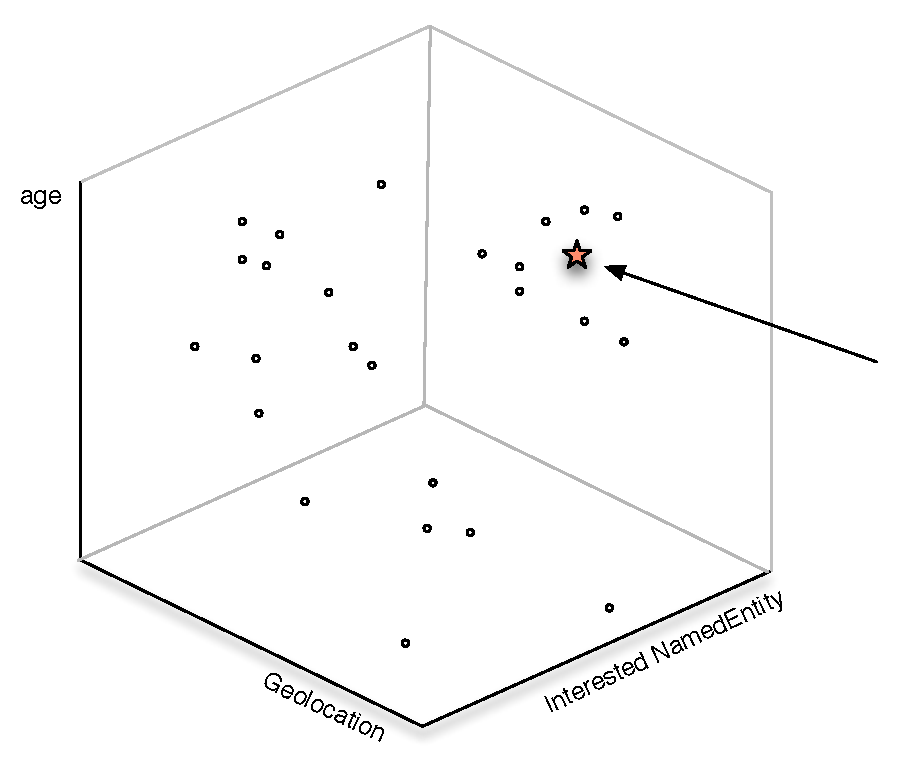
\includegraphics[scale=0.65, trim=0 10 0 0, clip=true] {featurespace.pdf}
\label{fig:featurespace}
\end{figure}

\chapter{Design}
\section{Overview}
The system proposed is one that places a synergy between the hardware and software at its heart, maximising not just all components of the underlying architecture but also ensuring that each component is utilised as efficiently as possible. The major components considered in this design:
\begin{itemize}
\item I/O bus
\item Main Memory
\item CPU cores
\item L3, L2, \& L1 cache lines
\end{itemize}
To understand how these components can be specialised, it is important to discuss how they work and what their role is in the overarching design of the system 
\subsection{Hardware components}
\subsubsection{I/O bus}
Like all internal system buses, the I/O bus is responsible for moving data from an auxiliary part of the computer to the CPU. I/O buses normally exclude main memory access and focus on components such as keyboard input, audio or, in the case interested in this project, network communication. Any data bound server instance like the one in question in this project requires extensive use of the networking interface, so much so that network is the primary bottleneck in such systems as IP packets are marshaled,copied and de-marshalled around the system using the I/O bus as its main \textit{highway} to all components. To ensure that this part of the system is as uncontended as possible, focus needs to be applied to reduce the overhead. In particular, the system keeps all marshalling and demarshalling as conservative as possible and uses the I/O bus to keep, as much as possible, this data away from main memory detours and interfaced directly with the CPU cores.
\subsubsection{CPU Cores}
In recent times we have seen Moores Law\footnote{A law describing the linear trend of core clock cycles/die-size over time} being upheld by the fact that, although clock speeds on single dies are plateauing due to physical constraints of heating and fixed atomic size, the number of clock cycles in a given CPU is still increasing due the addition of multiple cores on the same physical die. The Intel i7 CPU for example is fitted with up to 8 cores on a single die. Moreover, modern servers can be found with multiple CPU's means that upward of 24 cores can be found in modern systems.

Traditional procedural programming is still possible on such architecture but will be limited to a single core. Within a multitasking environment such a design is ok but when considering a single server instance responsible for a single task, threading or multi process design needs to be considered. A common technique is to use the threading model that conceptually isolates a unit of atomic work to occur concurrently with other threads. In a typical web server for example, the threading policy needs to be carefully tuned to obtain the maximum performance. Too few and the system is under utilised whilst too many results in contentious context switching. The problem with the threading model is it does not really reflect with is happening in the underlying hardware. Under the hood, processing is signaled using interrupts\footnote{In fact threading is achieved by \textit{multiplexing} these interrupts so that the illusion of atomic and concurrent units of work can be achieved} which tell the cpu which execution address to jump to next when IO events are received. The only real concurrent unit of work in a computer is what is actually executing on a CPU core at any one time. As such, the threading policy of this system should be such to mimic this behavior - 1 thread for each CPU\footnote{Ideally using thread affinity where the OS is instructed to only execute a given thread on a given core} with an event driven methodology to reflect the interrupt nature of the supporting buses.

\subsubsection{Main Memory and Caching}
\floatsetup[figure]{capposition=bottom}
\begin{figure}[h]
\centering
\caption{Illustration of the different cache visibilities based on a 2 CPU, 4 core setup. Visibility flows downward}
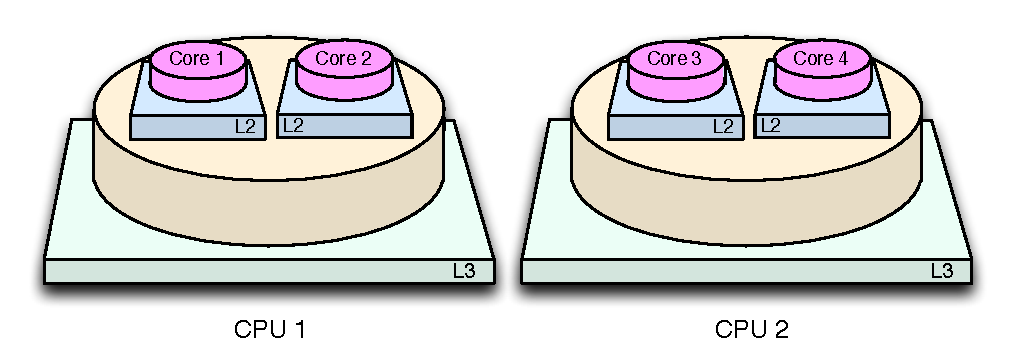
\includegraphics[scale=0.65] {cachelevels.pdf}
\label{fig:corecachedesign}
\end{figure}
Modern CPU's gain extensive performance improvements by using dedicated caching that sits on top of the processing units. These small but extremely fast memory elements sit directly within the CPU die allowing for frequently required data to be accessed at a fraction of the cost of accessing main memory. Caches map main memory in the form of cache lines that are contiguous areas that exploit both temporal (items used at time \(t\) are likely to be used at time \(t+1\)) and spatial locality (items located near each other are likely to be used at a similar time). Data of a cache line is moved from slow main memory into fast cache memory as it is being accessed. To optimise it's use of memory, the system needs to exploit the locality principles of the cache lines, avoiding cache misses and keeping data as close to the CPU for as long as possible. 

The downside with such design is that when data is sitting in cache lines, it is not guaranteed to be visible in other parts of the system. Data stored in the L2 cache of Core 1 of Figure \ref{fig:corecachedesign} cannot be seen in Core 2. Furthermore, data in the L3 cache of Core 3 cannot be seen by Core 2. Consequently, care has to be taken to set up correct memory barriers\footnote{In java for example, memory barriers are created using the \texttt{volatile} \& \texttt{sychronized} keywords and the \texttt{Sync} primatives from the concurrency package} when data is needed to be flushed back into main memory for other cores to see it.

\floatsetup[figure]{capposition=bottom,capbesideposition={top,right}}
\begin{figure}[h!]
\centering
\caption{Although there are multiple cache lines present in modern designs, as observed here the real speed benefit is avoiding main memory and as such this is the focus in this project.}
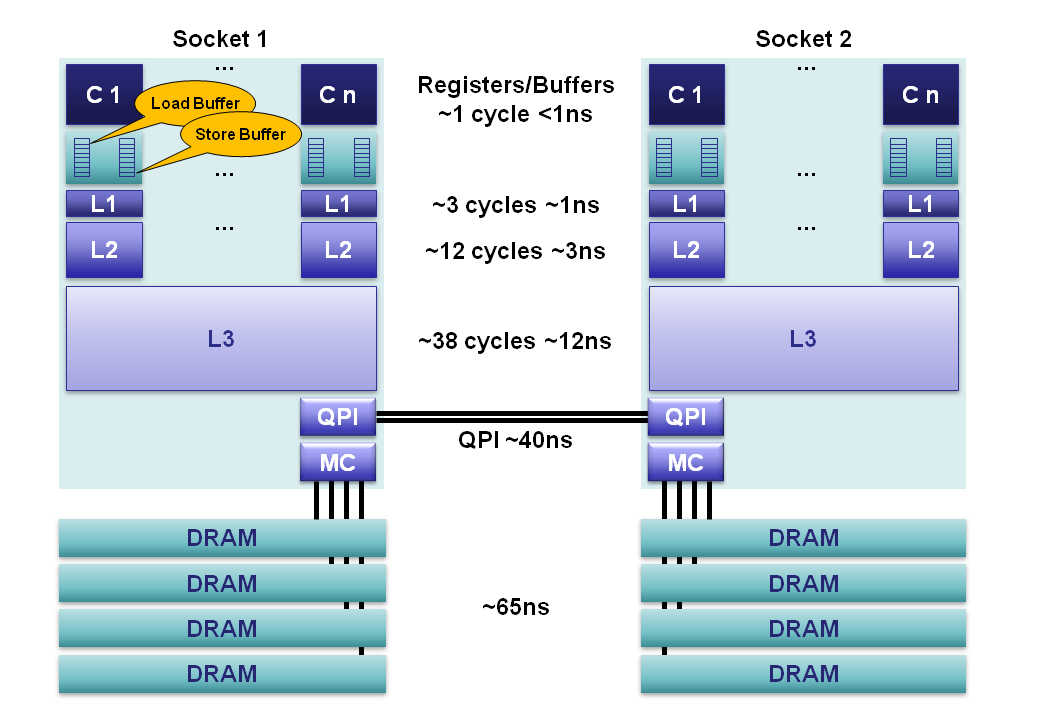
\includegraphics[scale=0.5] {cachelinespeed.png}
\label{fig:cachelinespeeds}
\end{figure}
Another consideration that's worth highlighting is that within managed virtual environments such as java, although all these components can be exploited using care consideration of the JVM contracts, nothing is guaranteed. The garbage collector in particular can become a catastrophic obstacle to such optimizations. Consequently, as much as possible, object pooling is used\footnote{Actually implemented transparently within the disruptor} and a precedence placed to avoid unnecessarily object creation.
\subsection{Software Architecture}
As previously mentioned, in order to optimize all the hardware components mentioned above an event driven design needs to be adopted, filing off to threading only to distribute the computational load across processing cores. To avoid the OS from scheduling another thread to a core whilst being worked on and thereby invalidating the caches, the number of threads is equal to \(-1\) the number of cores in the system\footnote{-1 is used to dedicate a core to the main scheduling thread of the system that deal with the IO coordination}.Once events have been handed over to a specific core, the thread that owns the event also \textit{owns} its visibility completely. That is to say that no other thread is expected to have read or write access to it whilst in this core's care. This allows the application to enforce locality benefits in the data without worrying about visibility to other threads and thus providing a setting that minimises the copying of cache lines to and from main memory and satisfies the desire to keep data as close to the Core as possible. When the core is finished with the event, a model of releasing ownership of a collection of events at once is adopted by \textit{pushing} these events downstream to another component where visibility is required. 

To facilitate the movement of these events from the input stream into the care of dedicated cores and finally, back into main memory, the use of the disruptor queues already mentioned is selected. Note only are these queues lightening fast but they also put in place the required memory barriers mentioned to, like a runner in a relay, pass off ownership of the event once it is finished with and providing the necessary visibility guarantees. Another side effect of this design, as will be seen, is that it is completely lockless, only relying on the CAS operations in the disruptor under busy load. Furthermore, there is only one custom \texttt{volatile} variable when running the system in \textit{Sync} mode. A rough architecture plan of the system is presented in Figure \ref{fig:architectureoverview}

\floatsetup[figure]{capposition=bottom,capbesideposition={top,right}}
\begin{figure}[h!]
\centering
\caption{The main modules and data flows of the system}
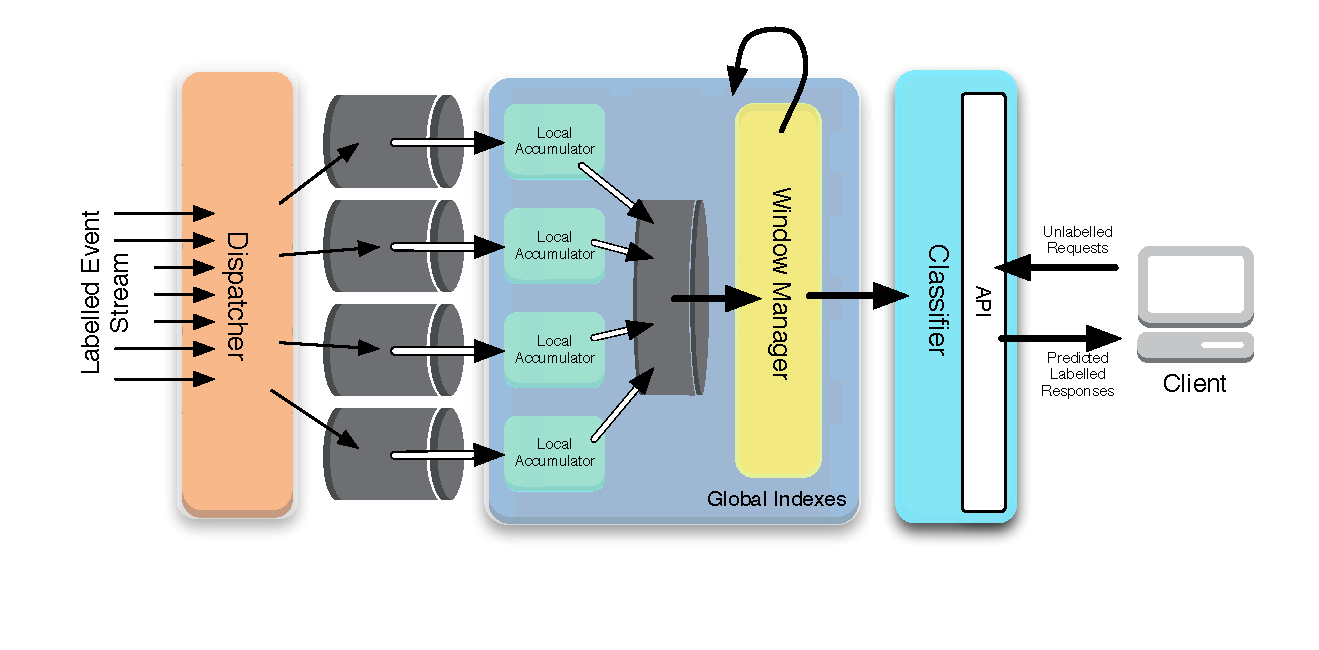
\includegraphics[scale=0.72, trim=35 50 0 13, clip=true] {architectureoverview.pdf}
\label{fig:architectureoverview}
\end{figure}
Events flow into the system and feed into the \textbf{Dispatcher} module by a single main thread. Here the events are randomly pushed into a series of disruptor queues, one for each CPU core using a simple uniform distribution. Each disruptor can be thought of as defining the work queue for each core whilst a dedicated thread associated with each one, consumes events one at a time. These worker threads then construct an accumulated view of a so called window of events. To aid in this, the \textbf{Accumulator} module exposes a highly cache efficient data structure that each thread has a \textit{local} instance of. These local instances are completely owned by each thread permitting both read and write operations and exist to fully exploit the cachelines of the underlying associated core. In order to maximise temporal locality, a shared \textit{global} index that can be used within the local accumulator so that more long term insights into the data can be shared across threads. To avoid unnecessarily cache flushes, this shared instance is completely immutable allowing only read access across the workers. Enforced using \texttt{final} declarations, data access from the global indexes can be essentially copied into the cache lines of each worker thread, maintaining the single ownership properties required of the worker data accesses - In this respect, the global index can be thought of as a read only instance that each thread has a copy of\footnote{When a worker accesses an item in the global index, the OS is free to copy the data into the local cache of whatever core the thread is assigned to}.

Once a window of events has been processed, the accumulated view is then pushed back into the main thread via the use of a single shared disruptor queue. The main thread then consumes these accumulated events and aggregates them together using a \textbf{Manager Manager}. This module takes each of the accumulated events and combines them into a single \textit{window} which represents a combined view of the data for a particular interval of time. As the accumulator threads push more and more windows into the manager, so it also keeps track of each interval, accumulating further to produce a single overarching representation of all accumulator windows and intervals. This serves as the main aggregated model of the system. This aggregated model is not only exposed to the \textbf{Classifier} to produce predicted labels to unseen events, but also back into the global accumulator so that the worker threads can profit from this longer sighted view of the data.

\subsection{Execution Modes}
To coordinate the determination of when a window of events has been processed the system uses a time expiration rather than a number of samples policy. The reason is that it parallels better the temporal nature of the window and makes the aggregation stage in the window manager easier to implement. Consequently, There needs to be a protocol for determining when the window has expired. There are 2 modes of execution. 
\subsubsection{Async}
\begin{figure}[h!]
\centering
	\begin{subfigure}[t]{2 in}
		\centering
		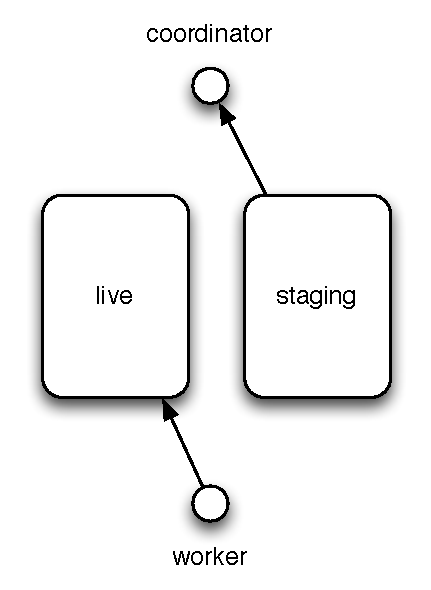
\includegraphics[scale=0.7]{async-mode1.pdf}
		\caption{\(t\)}\label{fig:asyncmode.t}		
	\end{subfigure}
	\begin{subfigure}[t]{2 in}
		\centering
		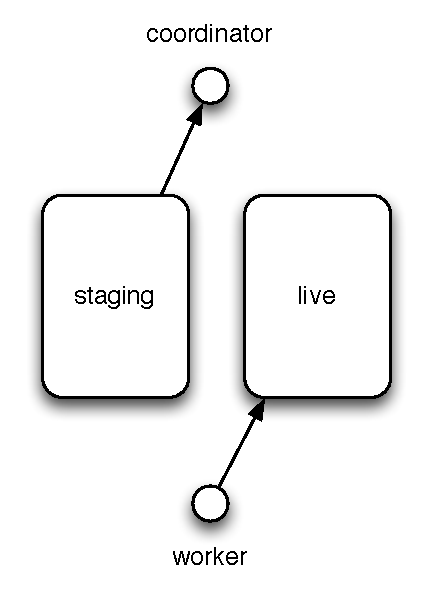
\includegraphics[scale=0.7]{async-mode2.pdf}
		\caption{\(t+1\)}\label{fig:asyncmode.tplus1}		
	\end{subfigure}
	\caption{How ownership of the accumulators change during the end of an interval}
\end{figure}
This is the most simplest mechanism to implement and revolves around a coordinator thread that, for the most part just sleeps. Every \(t\) seconds it wakes up and proceeds to read the contents of each accumulator, copying it into main memory before sending it into the window manager. The difficulty in this approach is that case needs to be taken when reading from the accumulator as this process not only needs to be visible (This is data owned by another thread and therefore offers no guarantees that the data will be in main memory and not on a cache line somewhere) but also atomic. Whilst we are reading from the accumulator we cant have that worker also updating it at the same time else data corruption becomes a risk. Consequently, if we use synchronization to coordinate the access any advantages of cache optimization are negated as the implicit memory barrier that comes with such locking will cause all writes to be written back into main memory, essentially throttling the event processing of the system. 

To avoid this, a setup up borrowed from \textit{hot-cold} DR topologies of server cluster is adopted where 2 copies exist of each local accumulator - one live and one staging. The purpose is that only one of these accumulators is owned by the worker thread. When the coordinator thread wakes up, it switches the live to staging and vice versa meaning that the worker thread relinquishes sole ownership of the live accumulator and takes on the staging one. Once the live accumulator is now staging, the coordinator thread can safely and atomically access the data in the accumulator. This can be implemented using just a single \texttt{volatile} bit mask that determines which accumulator is live. 
\subsubsection{Sync}
The other execution mode is one where there is no coordinator thread. Each worker is responsible for determining when a window is ready and the accumulated event should be pushed downstream as part of its actual processing task. This means there is no ownership transfer or extra memory impacting accumulator copies. One potential drawback of this approach is that, if there are no events in the system, the thread cannot check to see whether it current accumulator has expired and window intervals can become stale. To combat this, \textit{heart beat} events are added by the dispatcher at the boundary of each interval to ensure timely expiration of windows occurs. Because the main copying of the accumulators into main memory is performed on the work thread itself, this approach leads to short pauses in the event stream at window  
\section{Naive Bayes}
Potentially any classifier could be used but, as there is a focus to optimize the model to exploit the cache lines, one that can form a model representation using simple counts is extremely useful. Addition of simple variables in a continuous array is something that is extremely cache friendly and, as such the Naive Bayes technique is a perfect fit. Naive bayes works by building a probabilistic model using prior and posterior combinations of feature value/label pairs under strict naive assumptions of independence. The idea is that, by building probability distributions from observed events, unseen classifications can be predicted by maximising the likelihood estimates from the built distribution of all classifications based on the unseen event's feature values. 

\[\hat{y}=\argmax_{k \in \{1,...,K\}} p(C_k)\prod_{i=1}^n p(x_i | C_k)\]

Framing the classifier as a personalised trending now predictor, the formula is changed slightly so that, instead of returning the classification with the maximum probability, the \(m\) top most probable classes. By setting \(m=1\) this functions the same as the original \(\argmax\) revision. 

\[\hat{y_j}= p(C_j)\prod_{i=1}^n p(x_i | C_j))\]
\[\text{Without loss of generality and assuming that }  \hat{y_j} \geq \hat{y_{j'}} \text{ if } j < j'.\]
\[\mathbf{\hat{y}} = (\hat{y}_1, ..., \hat{y}_m) \text{ where } m \leq K\]
The prior \(p(C_j)\) term captures the traditional trending now function whereas the posterior \(p(x_i | C_j)\) captures the personalised extension.\\\\ There is an issue with the above in that, when dealing with features, the probabilities can approach zero very quickly resulting in underflow even when considering 64bit floating point values. To handle this, instead of taking the product of the probabilities, the ranking can be performed in log space where the sum of the log of the probabilities is used:

\[\hat{y_j}= \log p(C_j) + \sum_{i=1}^n \log p(x_i | C_j))\]
To build the probability distribution using an accumulator methodology is simple. When a labelled event is observed, an accumulator slot is referenced based on the classification value (to capture the prior) and one for each discrete feature value / classification pairing (capturing the posterior). The values in each of this slots is then incremented by 1. The probability for each prior term is then the total number of events seen of each classification value over the total number of events and the posterior terms is calculated as the total number of events seen of each feature/classification pairing over the total number of events of that particular class. Because of this setting, the classifier is also capable of predicting multi-class classification tasks.

\begin{figure}[h!]
\begin{subfigure}[t]{2 in}
\[p(C_k) = \frac{\nu(C_k)}{\sum_{i} \nu(C_i)}\]
\caption{Prior term calculation}
\end{subfigure}
\begin{subfigure}[t]{2 in}
\[p(x_i | C_k) = \frac{\nu(x_i | C_k)}{\nu(C_k)}\]
\caption{Posterior term calculation}
\end{subfigure}
\end{figure}
For continuous values, distributions can be assumed to represent probability density functions. In the case of a normal distribution, for a given continuous feature or classification type, the prior and posteriors can be estimated by building online streamed based mean and standard deviations based on the event stream. 

\begin{figure}[h!]
\begin{subfigure}[t]{2.5 in}
\[p(C_k) = \frac{1}{\sigma(C)\sqrt{2\pi}}e^{-\frac{(C_k - \mu(C))^2}{2\sigma(C)^2}}\]
\caption{Prior term calculation}
\end{subfigure}
\begin{subfigure}[t]{2.5 in}
\[p(x_i | C_k) = \frac{1}{\sigma(C_k)\sqrt{2\pi}}e^{-\frac{(x_i - \mu(C_k))^2}{2\sigma(C_k)^2}}\]
\caption{Posterior term calculation}
\end{subfigure}
\end{figure}
As it is not possible to store all event data in memory, calculation of the \(\mu\) and \(\sigma\) variables needs to be conducted in an online fashion\footnote{This online version proposed by Knuth\cite{knuth-aop} is an adaption of Welford's online variance method and is used due to its better handling of overflow} where just 3 variables can be used to capture the distribution parameters (namely \(n\), \(\mu\) and \(M_2\)). Each variable can occupy a single slot in the accumulator and are stored sequentially to exploit the spatial locality of cache lines.

\captionsetup[subfigure]{labelfont=bf,textfont=normalfont,singlelinecheck=off,justification=centering,labelformat=simple, labelsep=colon}
\begin{figure}[h!]
\begin{subfigure}[t]{2.5 in}
\[\mu_{i+1} = \mu_i + \frac{(x_i - \mu_i)}{(n_i)}\]
\caption{Mean Calculation}
\end{subfigure}
\begin{subfigure}[t]{2.5 in}
\[M_{2_{i+1}} = M_{2_i} + (x_i - \mu_i)(x - \mu_{i+1})\]
\caption{Intrim Calculation}
\end{subfigure}
\begin{subfigure}[t]{2.5 in}
\[\sigma_i = \frac{M_{2_i}}{(n_i-1)}\]
\caption{Variance Calculation}
\end{subfigure}
\end{figure}

The classifier needs to also handle the scenario where certain events may not have all features present. Handling missing features is done explicitly by the model as the counts for neither the numerator or denominator are incremented, assuming that this event for this feature/classification has never been observed. Because of the assumption of independence between posteriors, such an approach is possible but it worth mentioning that if, on the training set only a few events occur with a given feature, then this posterior maybe greatly biased as the laws of big numbers will not be applicable. The assumption here is that events needing classification will also be drawn from the same distribution of missing features and thus such a bias will not effect the overall performance.
\section{IO}
In order for events to enter the system, a sensible IO strategy is needed not just to transport the bytes but also to deserialize them into a format that can be made sense of. This deserialising is a major bottleneck in any IO heavy system so care needs to be taken to ensure it is as efficient as possible
\subsection{Selectors}
As previously mentioned, the IO bus on modern architectures relies on interrupts that occur when data is available on the IO bus. In order to mimic this as much as possible, the system utilises the selector mechanism of *nix operating systems that approximates a 1-1 mapping between these interrupts and a kernal event from the OS. Java's NIO module provides an interface to this system. Furthermore, normally memory is indexed in java using a specialised heap that the GC can maintain. Traditionally, all data accessed within the JVM needs to be present in this heap but for networking, this means that data on the IO bus needs to first be copied into main memory prior to being processed. For the stream based methodology that this system utilises, this unnecessary detour not only adds extra transfer time as data is proxied through the heap but also puts extra burden on the garbage collector.
To limited this, advantage is taken of the off heap byte buffers of the NIO package. These abstractions ensure that data is taken directly from the network interface into the CPU for serialising, and thus avoids commuting to the heap.
\subsection{Protostuff}
Serialisation that governs data interchange needs to be defined so that a contract of how events can be passed from up stream producers into the system. As deserialising is one of the main overheads of any high throughput system, one that focuses on both flexibility and speed is paramount. Consequently, Google's protobuf\cite{googleprotobuf} format is provided using the protostuff extension as a default implementation\footnote{The application is capable of supporting any demarshalling technology via the generic \texttt{EventMarshalBuffer} interface}. This was chosen because of it's external schema design, variable length encoding and sequential byte stream support that aids in good cache utilisation. Unfortunately, protostuff does not support proper off heap byte buffers so an extension was specifically created to exploit this\footnote{Now contributed back into the protostuff project}.
\subsection{Transport}
There are two main IP protocols in wide use namely TCP and UDP. TCP allows data to sent into packets or windows of data where each packet needs to receive a checksum response to ensure that each packet has been received correctly. This provides delivery guarantees at the expense of extra communication and checksumming. UDP on the other hand transfers as a large stream of data which may or may not reach the target destination. Unlike TCP, although no guarantees can be made on whether data corruptness has occurred, UDP is free of the extra overhead and so, in theory, is faster. The system supports both mechanisms as, if corruption does occur with UDP, as this is a high throughput system running under big data load, such random permutations will not affect the underlying distributions too much\footnote{Assuming the environment is stable (such as within a datacenter) error rates should be relatively low}.
\section{WindowManager}
\floatsetup[figure]{capposition=bottom,capbesideposition={top,right}}
\begin{figure}[h!]
\centering
\caption{Illustration of how a new window interval arriving into the Window Manager will push out an older interval}
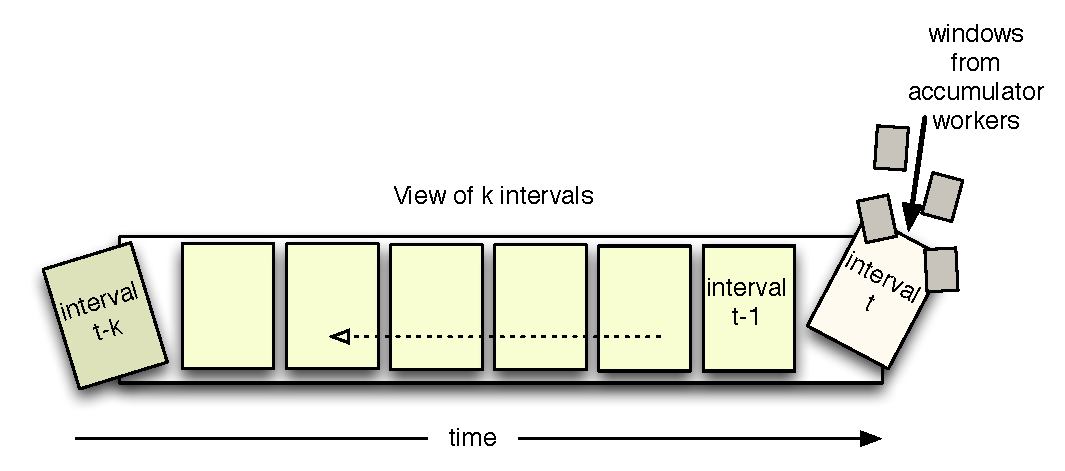
\includegraphics[scale=0.72, trim=0 0 0 12, clip=true] {window.pdf}
\label{fig:rollingwindow}
\end{figure}
The window manager is responsible for aggregating different event windows and intervals and controlling the expiration of each. It follows a rolling window design (see Figure \ref{fig:rollingwindow}) where by a view of \(k\) intervals of \(i\) time is maintained at any given moment. Each interval, created at time \(t\) is built from multiple windows from the accumulators which are combined together until the interval is no longer current at \(time = t+i\). At this point the interval is made immutable and a new interval created and set as current. 

The total view of the window manager is then maintained by a separate aggregated state that represents all the aggregated intervals together. For discrete features, whenever an interval at time \(t\) is added to the view, the prior and posterior counts of this new interval are summed together whilst, when interval \(t-k\) leaves the view, its counts are subtracted from the aggregated state. When dealing with continuous values, the parameters of the underlying models need to also be summed and subtracted. For the case of the normal distribution, the parameters are summed and subtracted using the following bias corrected equations:
\newpage
\begin{myequations}
\begin{equation}
\mu_c = \frac{n_1\mu_1 + n_2\mu_2}{n_1 + n_2}
\end{equation}
\begin{equation}
\sigma_c = \frac{(((n_1 -1) \sigma_1) + ((n_2-1) \sigma_2) + n_1(\mu_1 - \mu_c)^2) + n_2(\mu_2 - \mu_c)^2)}{n_c-1}
\end{equation}
\label{eq:combiningparamsadd}
\captionof{myequations}{Addition of normal distribution parameters for each windows/intervals}
\end{myequations}

\begin{myequations}
\begin{equation}
\mu_s = \frac{n_1\mu_1 - n_2\mu_2}{n_1 - n_2}
\end{equation}
\begin{equation}
\sigma_s = \frac{(((n_1 -1) \sigma_1) - ((n_2-1) \sigma_2) - n_1(\mu_1 - \mu_c)^2) - n_2(\mu_2 - \mu_c)^2)}{n_c-1}
\end{equation}
\label{eq:combiningparamssub}
\captionof{myequations}{Subtraction of normal distribution parameters for each windows/intervals}
\end{myequations}
 
\section{Accumulators}
The accumulators are specifically tailored data structures used to optimize the cache layouts of the underlying hardware and represents the cornerstone of aggregating events into the accumulated models and make up each window. Essentially, they represents an indexable sequence of memory that focuses on structuring the indexes in such a way to exploit both the temporal and spatial qualities of the cache lines. This abstraction of position and value is the heart of the structure. The accumulator is essentially an expanding tree that indexes a leaf based on a given slot number that references the required value. Each leaf is actually a primitive array of integers created with a length equal to that of the cache line of the underlying CPU cores. The values that these slot numbers refer to relate to the variables needed for the naive bayes classifier and are determined by different lookup strategies according to the instance type of the accumulator. \\
\floatsetup[figure]{capposition=bottom,capbesideposition={top,right}}
\begin{figure}[h!]
\centering
\caption{shows a trival example of indexing slot 10. Note that the left most outer leaf is not assigned demonstrating the expanding and space saving design}
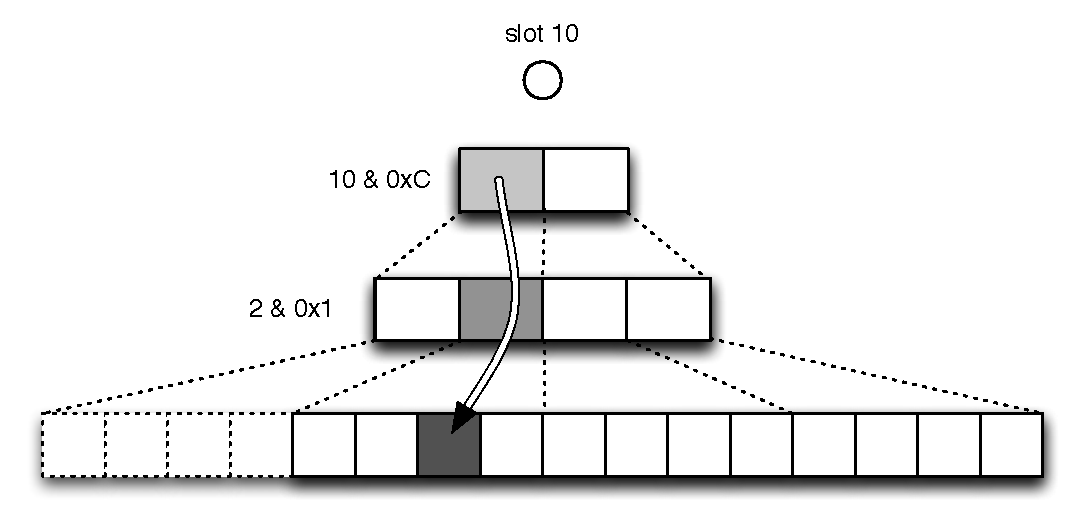
\includegraphics[scale=0.72, trim=0 0 0 12, clip=true] {accumulator-lookup.pdf}
\label{fig:accumulator-lookup}
\end{figure}

The idea being that, most frequently accessed data sits together in the same leaf array and therefore the same cache line, optimising for cache hits and avoiding fetches into main memory. The structure grows as more slots are needed so that large and unnecessary allocation of array space can be avoided. To obtain a slot in the accumulator, its location in the tree is determined using a 3 level accumulator line structure where each line can be considered a depth in the tree. which branch at each level is then determined using the high order bit terms of the slot value. This results in slot numbers where the low order terms are similar to be more likely to reside in the same cache line.

\subsection{Index Instances}
For each worker thread there exists a dedicated accumulator instance that it has complete ownership of. All reads and writes are solely for the purposes of the owner thread which allows the cache optimisations detailed previously to function. In the naive bayes framing, a particular prior or posterior pairing needs be assigned to a particular slot in order to index into the accumulator in a deterministic manner. This lookup follows a hierarchical model where a given feature or feature/classification pairing is first checked in a global instance. If the global instance returns a slot number then this is used to index the accumulator - if not, a local instance is used.
\subsubsection{Local Instance}
Local mode indexes as ones that are completely unique to a given worker and are mutable in that new indexes cannot be assigned. If a given feature or feature/classification pairing is not present in the index, it is subsequently added against the next available slot in the accumulator. When slots are determined from local indexes, only spatial locality can be exploited as, being on the critical event stream path of the system, they need to function as quickly as possible.
\subsubsection{Global Instance}
This is a read only shared instance that all worker have access to. After every time the window manager is updated with a new interval, indexes for all seen required variables (both for discrete and continuous feature types) are re computed based on a ranking of how frequently they have been seen. If \(p(x_1 | C_1)\) is the most observed posterior and \(p(x_2 | C_2)\) is the second most observed, then these will be reshuffled in to slots 0 and 1 respectively. By performing this reordering once every interval, temporal locality can be exploited by referencing the updates into the same leaf and therefore same underlying cache line. As this is a shared instance, a single \texttt{volatile} reference is shared amongst all workers and, as it is read only, no explicit locking is required, just the visibility guarantees. On each interval update, the window manager generates a new global index and reassigns the \texttt{volatile} reference to this new one for all the workers to see. To avoid boundary cases during updates, the global reference maintains its own namespace in the accumulators. This means that a given variable may be indexed from both a local and global slot and, as such, when constructing prior and posterior probability distributions, both need to be considered.

\floatsetup[figure]{capposition=bottom,capbesideposition={top,right}}
\begin{figure}[h!]
\centering
\caption{Show's the data flow between the global and local indexes and the local accumulators and window manager. Blackened arrows represent data pushes whereas grey arrows represent data fetches}
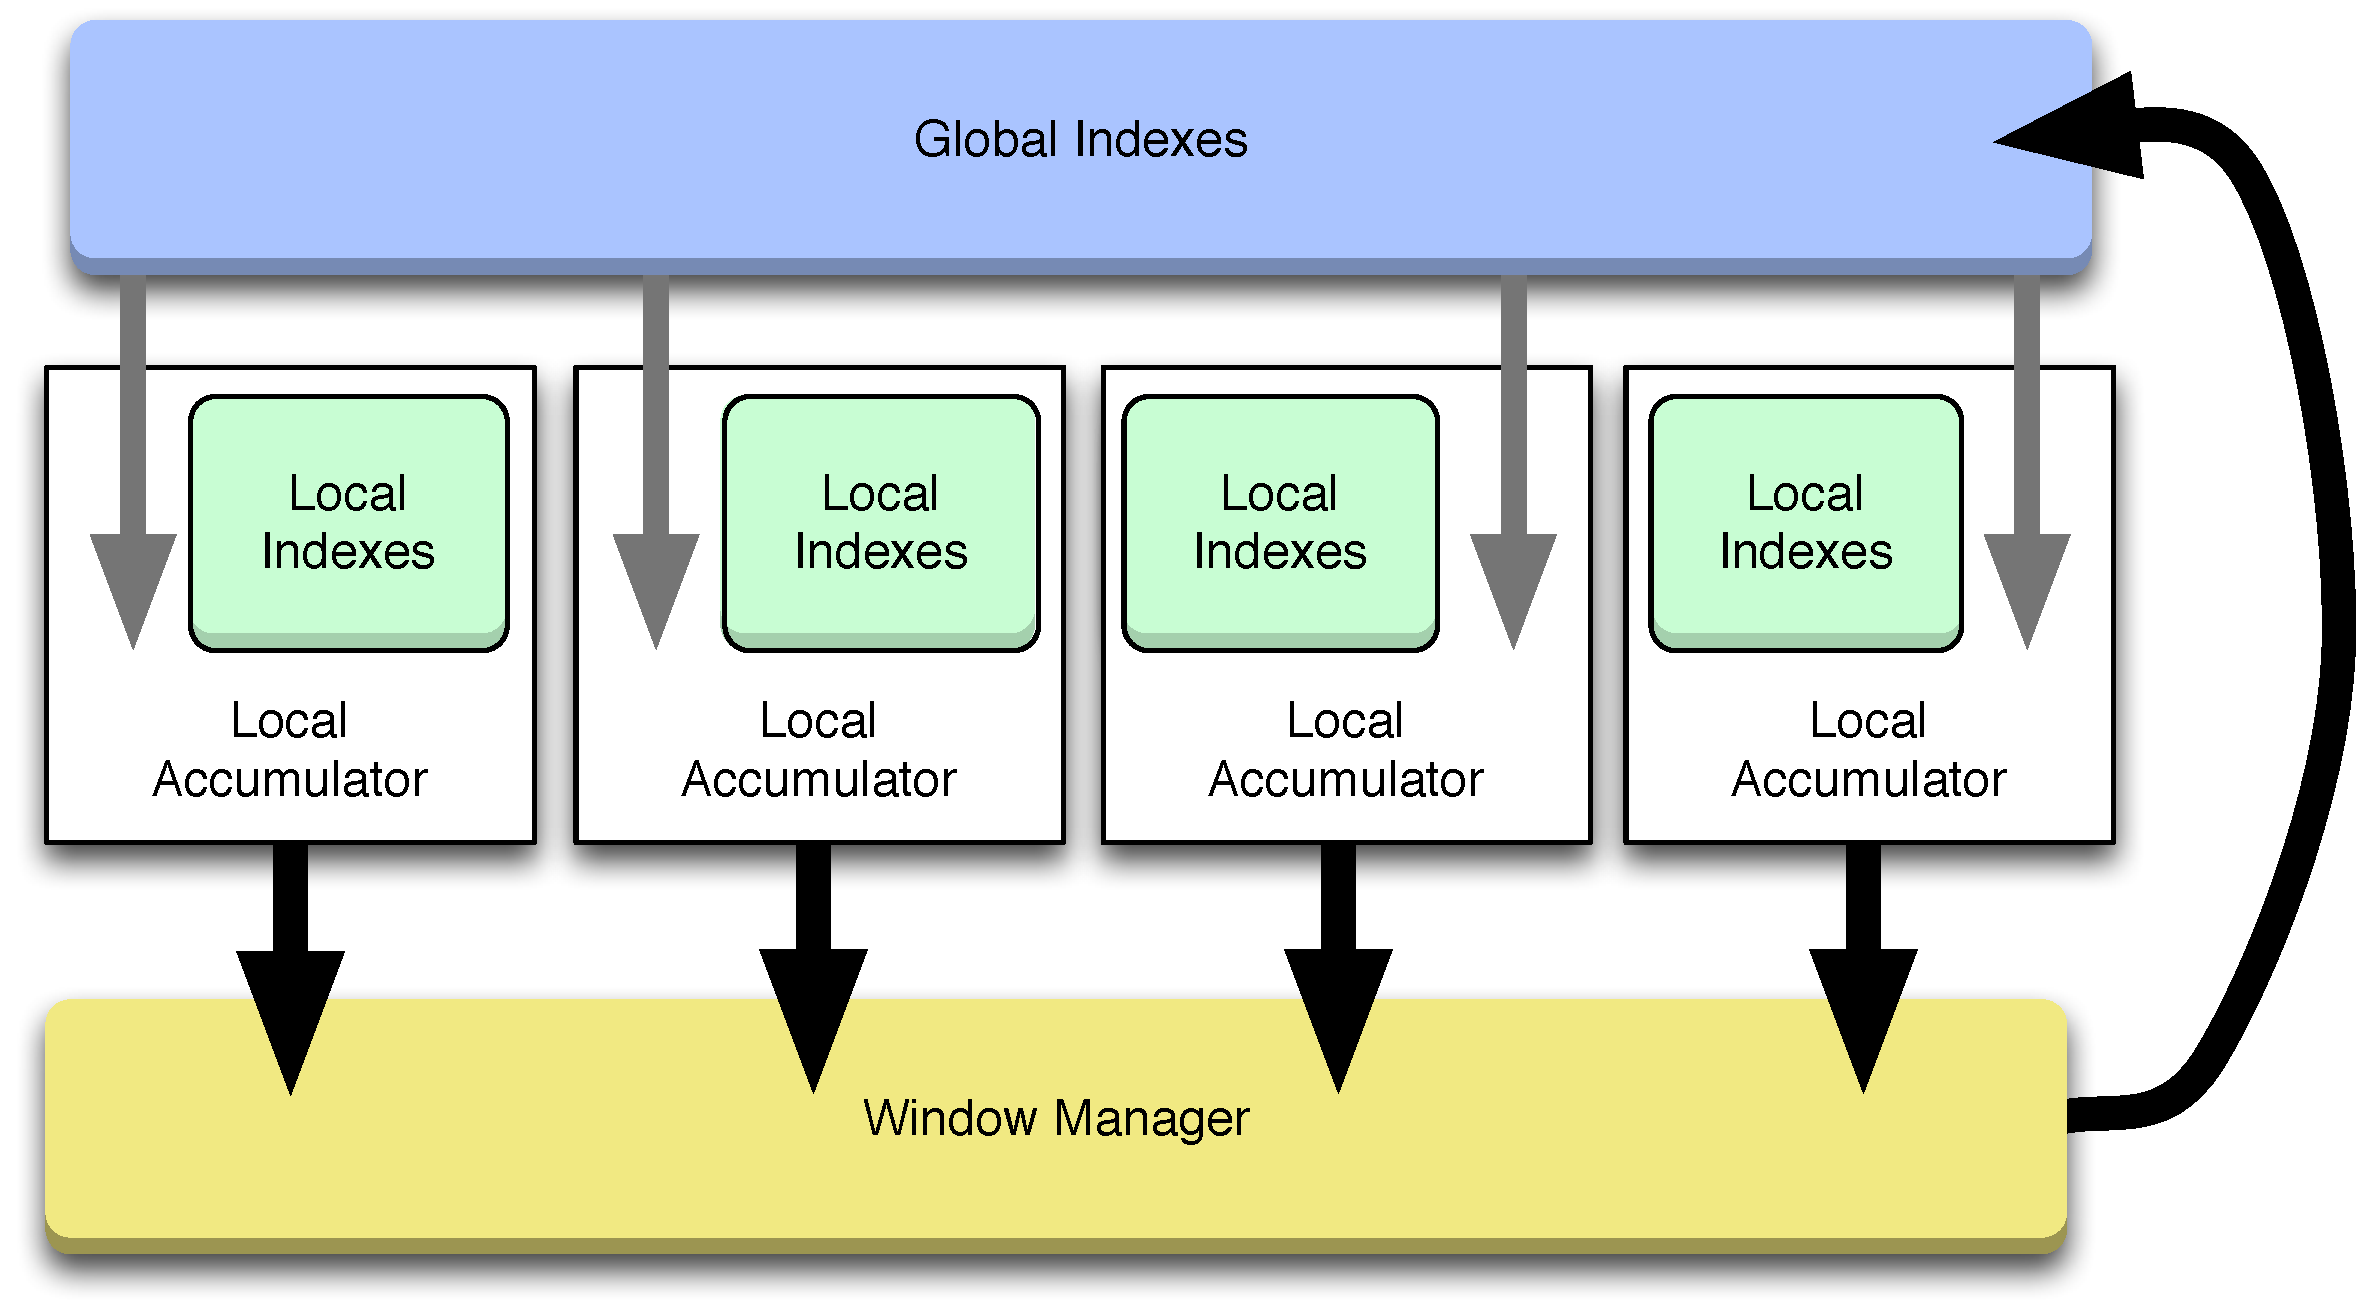
\includegraphics[scale=0.35, trim=0 0 0 12, clip=true] {indexes.pdf}
\label{fig:indexes}
\end{figure}

\chapter{Implementation}
\VerbatimFootnotes
\section{Overview}
The system is implemented on top of the java programming language and virtual machine allowing it to execute on commodity hardware and OS even if the certain architectural paradigms the system optimizes for are absent. The name of RCE (Realtime Classification Engine) has been adopted as a working title for the system. \\A number of design patterns are carefully chosen for this implementation in order to alleviate some of the thread safety and IO concerns that naturally arise in such a concurrent system. As this is an event driven system, there needs to be a clear distinction between data and logic. 
\subsection{Data}
Data is stored throughout in dumb 'model' objects \footnote{designated within com.haines.ml.rce.*.model.* packages} which can be considered to be the events. These lightweight objects contain no business logic and exist to simply define the schema of data used in the application. For the most part, this data is immutable and final to ensure that data is visible and sharable across threads. Areas where contentious access occurs, namely within the shared global accumulator state (\verb|NaiveBayesGlobalIndexes|), are handled with great consideration and, due to the live/staging methodologies already discussed, safe updating of such shared data need only use volatile variables\footnote{One example of this is in the shared \verb|VolatileNaiveBayesGlobalIndexesProvider| instance.}. 

The model objects that exist outside of the application domain that relate to the public API of the system are coded to interfaces. This allows any of the application code to be agnostic of serialization concerns of the implementing classes used to move the data from external clients in and out of the public API. The MVC patten is one that helps enforce this separation and is adopted throughout this application. Normally large scale applications take this concept of API and domain isolation further via the inclusion of a mapping layer that converts serialization objects from the controller into the application domain. However as such a technique incurs significant costs both in the copying of data between objects and the extra memory footprint for the garbage collector to work with, this coding to interface approach is deemed a sensible compromise. 

When indexing data the gnu trove libraries are used in place of the java JDK collections framework to allow primitive values to be stored directly without the unnecessarily need to create wrapper objects that add to the footprint of the garbage collector process.

In the rare scenarios where data needs to be transformed (i.e not changed but projected into a different structure), the delegation patten\cite{design-patterns} is used to transparently perform this task. The \verb|RCEConfig| object is an example of this.
\subsection{Logic}
Actual business logic is stored in classes in either two ways. More often than not, \verb|Service| classes are used which contain no state and are designed to be instantiated once as a shared global instance\footnote{although not implemented via the Singleton anti-pattern}. These instances then operate on supplied data model objects and coordinate flow based on the business logic each Service is responsible for. Due to the immutable contract of the model classes, some further classes where the control of data under contentious access is paramount, data and business logic is combined in a dedicated class. The Accumulators for instance contain both data (the accumulator structure) and business logic (how global and local indexes interact for example). These classes break this rule of data and execution logic separation to ensure thread safety without requiring on costly object allocation. 
\subsection{Application Instantiation}
Because certain objects have affinity to specific threads(like the \verb|Accumulator| and supporting classes) whilst others are more global in nature (\verb|Service| instances), a patten is required to manage instantiation and wiring of these instances. For this, inversion of control\cite{ioc} is adopted where instances assume nothing about implementations and life cycles of their dependent components whilst a single IOC factory is then responsible for the instantiation and injection of an instance and its components. In the case of this project, the \verb|RCEApplicationFactory| provides the main entry point into the construction of the application. Originally Google's Guice\cite{guice} was planned to be used to handle this task but, due to the thready affinity requirements of large parts of the system, this became unwieldy to manage \footnote{See \verb|GuiceRCEApplicationFactory| and corresponding \verb|RCEConfigConfiguredInitiationModule| for an idea of the complexities}. Consequently, a bespoke IOC factory was implemented catering to the novel requirements of the system design whilst the \verb|ServiceLoader| framework of the JDK is used to bootstrap the construction. The package \verb|com.haines.ml.rce.main.factory| contains the IOC factories used to instantiate and configure the system which will be discussed in more detail later in this chapter.
\subsection{DataStructures}
Apart from the bespoke structures already discussed, whenever the system needs to communicate a number of specific instances to downstream components, it does so using the most minimal building block of the Java collections API namely the \verb|Iterable| class. The reason for this is two fold. Firstly, the interface only allows read access which, even if implementing collections don't explicitly enforce immutability, the design of this API keeps access in a read only and thus thread safe manner by default\footnote{Technically care still needs to be taken to ensure visibility}. Secondly and more importantly it enables on demand manipulation of data in a functional manner. This can be extremely useful and performant especially in an event driven system such as this. Data that passes through may need to be manipulated in certain scenarios to downstream actors. Data could be manipulated in anticipation but what if downstream components dont need to use such data? This extra work would have been performed unnecessarily. A better approach is to wrap the iterable so that whenever a forEach construct is applied to it, on demand the translation function is executed during iteration. \\
Prior to version 8 Java provides no natively functional constructs but this doesn't mean that such paradigms are impossible to implement. Because the system is designed to be compatible with as wide an infrastructure as possible, enforcing java 8 was something felt to be avoided. therefore, static and final instances of Google's Function class from the guava libraries are used to mimic functional behavior and reap its on demand benefits. Where multiple invocations of a given iterable are possible, to reduce the repeated invocation of a costly function, the \verb|com.haines.ml.util.CachedIterable| class is provided to wrap functional iterables to cache their results.

\section{Maven Modules}
The system utilizes a number of different libraries and adopts a number of conceptual logical components. To manage the dependency tree's, versioning, lifecycles and build of these components, the apache maven project\cite{maven} is used. Maven allows versioned dependencies to be specified in an XML pom file and manages the build life cycle, including testing and packaging of various artifacts that make up the system. As the application is relative large, the reactor functionality of maven is used to help define atomic units of functionality into separate modules that make up the application. 

\floatsetup[figure]{capposition=bottom,capbesideposition={top,right}}
\begin{figure}[h!]
\centering
\caption{The main component structure of the RCE application}
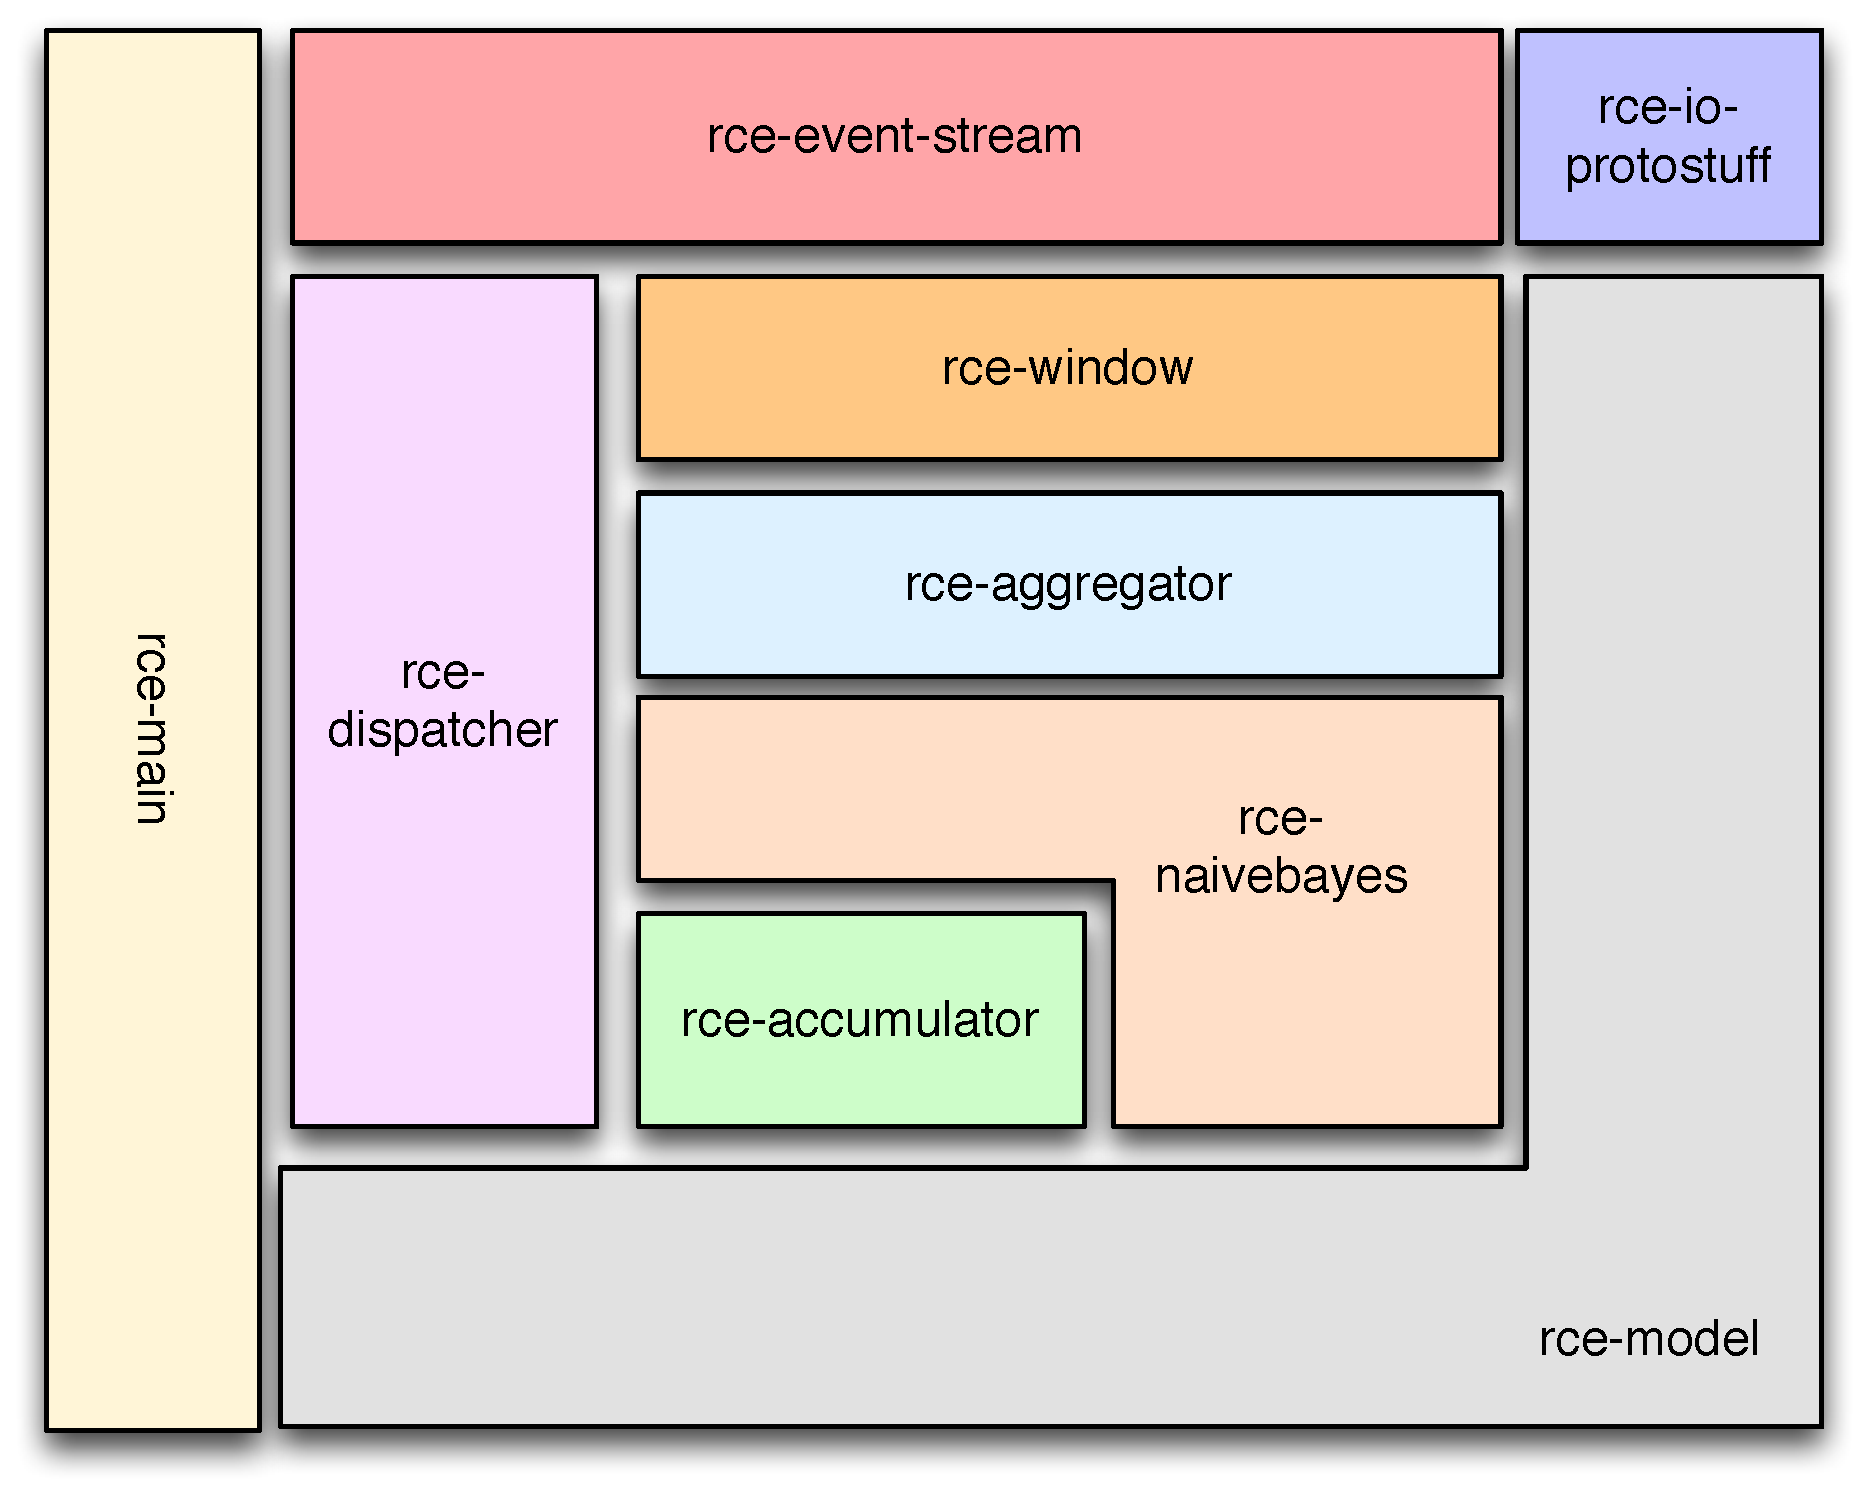
\includegraphics[scale=0.35, trim=0 0 0 0, clip=true] {reactor-layout.pdf}
\label{fig:indexes}
\end{figure}

Two further modules exist within the reactor build that form the basis of acceptance testing of the application. \verb|rce-performance-test| is responsible for testing the classification performance whilst \verb|rce-loadtest| is tasked with performance throughput and latency analysis of the system.

\subsection{The Components}
\subsubsection[rce-model]{rce-model\protect\footnote{It is called \textit{model} to mimic the MVC definition that this component represents although it is understood that this might cause confusions when considering the implications of such a name in the machine learning universe}}
This defines the data encapsulation interfaces or domain objects that all execution of the system interact with. That is not to say that all model objects are defined in this component. Other's exist to provide specific domain definitions for givens modules to function (like \verb|NaiveBayesDistributionCounts|) but all cross concern domain objects are defined here. Further to this, interfaces for some of the eventing mechanisms are also defined here such as \verb|EventConsumer| so that all high level components utilise these global definitions without needing to be concerned about their implementation. This functions are the data flow interface that allows modules to communicate with each other.

\subsubsection{rce-dispatcher}
This vertical module encapsulates all the queue and event driven paradigms that the other horizontal modules utilise. It uses provides an abstraction to the disruptor library to deal with message coordination along with the main thread affinity dispatcher to push events into dedicated CPU's.

\subsubsection{rce-accumulator}
This defines the core accumulator datastructure with indexing types. When an event is received, which slots are to implemented from the indexes is determined by implementations of the \verb|AccumulatorLookupStrategy| interface. Using this design keeps the framework completely agnostic from it's application usage. Currently a naive bayes implementation exists to convert an event into the slots required to increment it's prior and posterior counts but this need not be the only model employed. A spatial model such as Radial Basis Functions would also fit well in this design along with an application completely divergent from an ML classification task\footnote{Consider a application used for alerting that warns if too many failures of a particular type have occurred.}\\
To facilitate the different usages of discrete verses distribution based continuous accumulation, \verb|FeatureHandler| and \verb|ClassificationHandler| interfaces are provided that self as the public API interaction with the accumulators along with two provided implementations namely \verb|SequentialDistributionFeatureHandler| and\\ \verb|DiscreteLookupAccumulatorHandler|\footnote{A third is also provided called \verb|BucketedFeatureHandler| that is discussed more in the Future Work chapter}

\subsubsection{rce-naivebayes}
This provides the naive bayes implementation for the classification task of this system. It includes a \verb|RONaiveBayesMapBasedLookupStrategy| implementation for determining which slots should be incremented for a given event. It also defines the classification service to classify unseen events using probability models defined by implementations of \verb|NaiveBayesProbabilitiesProvider|. \\There is a scenario where the model may not have seen any occurrences of a given feature value and therefore it's posterior probability will be zero\footnote{More specifically this will be \(\infty\) once the \(\log\) is taken} and thus the final likelihood probability will be evaluated to zero. To tackle this, a nominal probability is defined that is \(> 0\) that acts as a lower bound of any probability calculation to ensure that one posterior can't have too great an influence on the overall outcome.  

\subsubsection{rce-aggregator}
This provides logic to aggregate multiple naive bayes counts together. This serves as the tooling for not only merging multiple local accumulator states together but also within the window manager as windows are added and removed.

\subsubsection{rce-window}
Provides the window manager implementation that uses the \verb|Aggregator| to add and subtract windows from it's internal state. The \verb|WindowManager| class is also a\\ \verb|NaiveBayesProbabilitiesProvider| that represents the probability model used when classifying.

\subsubsection{rce-event-stream}
This defines the controller and main processing loop of the system that takes events off the network bus, deserialises them and sends them on to the dispatcher.

\subsubsection{rce-io-protostuff}
Implements the domain model interfaces with protostuff serialising and deserialising instances which read directly off the bus rather than from the heap.

\subsubsection{rce-main}
Provides the IOC factory instances that actually build and configure the system. A main driver class for the application is also provided in the form of \verb|DefaultRCEApplication| but more bespoke invocations are possible such as the methodology used in the test cases as defined in \verb|RCEApplicationStartupTest|.

\section{Configuration}
The system uses two fundamental configuration mechanisms - ServiceLoader invocation of custom pluggable objects and JAXB defined XML\footnote{JAXB also supports other serialization formats such as JSON but the default format the system uses is XML} property files.

\subsubsection{ServiceLoader}
The java JDK contains a lightweight service provider loading facility named the ServiceLoader. The mechanism allows implementations of interfaces to be provided at runtime using definitions detailed in META-INF/service/* files as they appear on the runtime classpath. This allows additional behavior to be defined by simply including extra jars on the classpath and the ServiceLoader will reflectively instantiate them and add them into the IOC container. The system uses the ServiceLoader to allow 2 primary execution components to be extended or to provide pluggable additional functionality.\\
The first is the actual application container itself. This allows different ways of configuring the system to be programmatically defined which gives users the ability to completely customize the internals of how the system fits together. A number of 'building blocks' of abstract classes are provided that can aid in providing a default configuration of the system. The most specific class being\\ \verb|ProtostuffNaiveBayesRCEApplicationFactory| which users will need to extend to define the \verb|Schema| of the protostuff messages that form the (de)seriliasation protocol of the input API\footnote{see \verb|com.haines.ml.rce.main.factory.StaticProtostuffNaiveBayesRCEApplicationFactory| for an example of a concrete factory that only allows String based discrete feature and classification values}.\\

The other place the ServiceLoader is used is in defining how different features and classification types are handled. If \(f_1\) should use a discrete modeling whilst \(f_2\) uses a continuous normal distribution fitting, one can programmatically define this functionality by implementing \verb|FeatureHandlerRepositoryFactory| and adding the appropriate jar onto the classpath. 

\subsubsection{JAXB Config}
For more parameter based configuration such as window sizes, accumulator bit depth etc, JAXB defined XML files detail these properties. Config files are determined at the IOC container level such as via the driver commandline argument of \verb|configOverrideLocation|. A default-config.xml is provided to define sensible defaults that are used if a user specific configuration file is omitting all or part of the configuration property set.

\section{Testing}
There are 5 different test types that this project uses to verify semantic and performant correctness of the system. For all test types the Junit framework coordinates the test execution and integrates the results as part of the maven build configurations. Furthermore, the Cobertura code coverage tool can be invoked as part of the maven build using the \verb|site| target. This will produce reports detailing line-by-line coverage of tests see \ref{tab:coverage}
\begin{table}[h!]
\begin{tabular}{l*{6}{c}r}
Module              & No. Classes & No. Lines & Line Coverage & Branch Coverage & Complexity\footnote{Complexity an indication of how complex (no branch conditions) a module is. It uses the McCabe's cyclomatic code complexity routine\cite{mccabecc}} \\
\hline
rce-model & 28 & 168 & 0.762 & 0.706 & 1.638 \\
rce-io-protostuff & 2 & 381 & 0.858 & 0.739 & 4.55 \\
rce-dispatcher & 14 & 66 & 0.848 & 0.500 & 1.125 \\
rce-accumulator & 25 & 281 & 0.630 & 0.729 & 1.274 \\
rce-naivebayes & 59 & 646 & 0.749 & 0.591 & 1.717 \\
rce-aggregator & 3 & 68 & 0.735 & 0.700 & 1.600 \\
rce-window & 10 & 153 & 0.654 & 0.435 & 1.833 \\
rce-eventstream & 24 & 227 & 0.692 & 0.512 & 1.382 \\
rce-main & 57 & 524 & 0.761 & 0.551 & 1.423 \\
\end{tabular}
\caption{Code coverage of RCE application code base.}
\label{tab:coverage}
\end{table}

\subsection{Unit Tests}
For each conceptual unit of code (for the most part defined it's own file), a unit test exists that asserts the functional correctness of that component. Data used as input is either defined using test instances or via mocks provided by the mockito framework. Assertions are provided by the hamcrest library for more readable syntax.
\subsection{Functional Tests}
This suite of tests verifies that multiple instances of units of functionality within a single component or module interact with each other correctly, performing the correct semantic behaviour.
\subsection{Integration Tests}
This suite of tests verifies that various configurations of the entire system operate correctly. They are blanket tests that test the entire system is performing correctly at a broad level. In the system the \verb|RCEApplicationStartupTest| is such a test that verifies two configurations (UDP and TCP) start up and process a number of events without error. At this stage, no effort is made to ensure that the performance of the classifier is acceptable
\subsection{Performance Tests}
This test suite is responsible for ensuring that the performance of the system is acceptable. The basis of these tests is to use known labelled datasets (input with expected output) and partition them into two disjoint subsets each using a fixed ratio. The larger of the subsets is deemed the training set and is used to train the classifier by pushing events into the main input of the system. The remaining set, known as the test set, is then used to see how well the learned classifier does at predicting these remaining labelled instances. To further the accuracy of the test, the test is repeated a total of \(n\) times with different partitions of the training and test sets known as n-fold cross validation whilst multi-class performance is evaluated using a 1 vs rest scheme. A small framework has been built in \verb|rce-performance-test| that defines the these datasets, performs this type of testing and produces reporting (precision, recall, fmeasure and AUC metrics) along with ROC plots\footnote{see \verb|AbstractPerformanceTest| and the \verb|ReportGenerator| and \verb|ReportRenderer| class for details}. The 3 data sets are:

\subsubsection{Synthetic Dataset}
This test set (implemented in \verb|SyntheticTestDataset|) is synthetic in that a mixture model of defined fixed parameter normal distributions are used to generate feature values and their corresponding classification labels. In addition to the distributions, a uniform random process is added to simulate noise and ensure that the model generalises. The task of the classifier is to learn the underlying distributions so that when unseen samples from the mixture model are taken, the system can predict the class.\\ This test is used to help test how well the classifier functions as noise is increased in a controlled manner, provides a good setting for continous feature type tests and, as is a generator, the number of instances can be increased to a level required for the load tests, mentioned later on.
\floatsetup[figure]{capposition=bottom,capbesideposition={top,right}}
\begin{figure}[h!]
\centering
\caption{An example of a 1 feature, 3 class mixture distribution model where probability densities are shown according to the class (colour). When adding more features, the distribution mixtures fan out into more dimensions according to their hyper parameters}
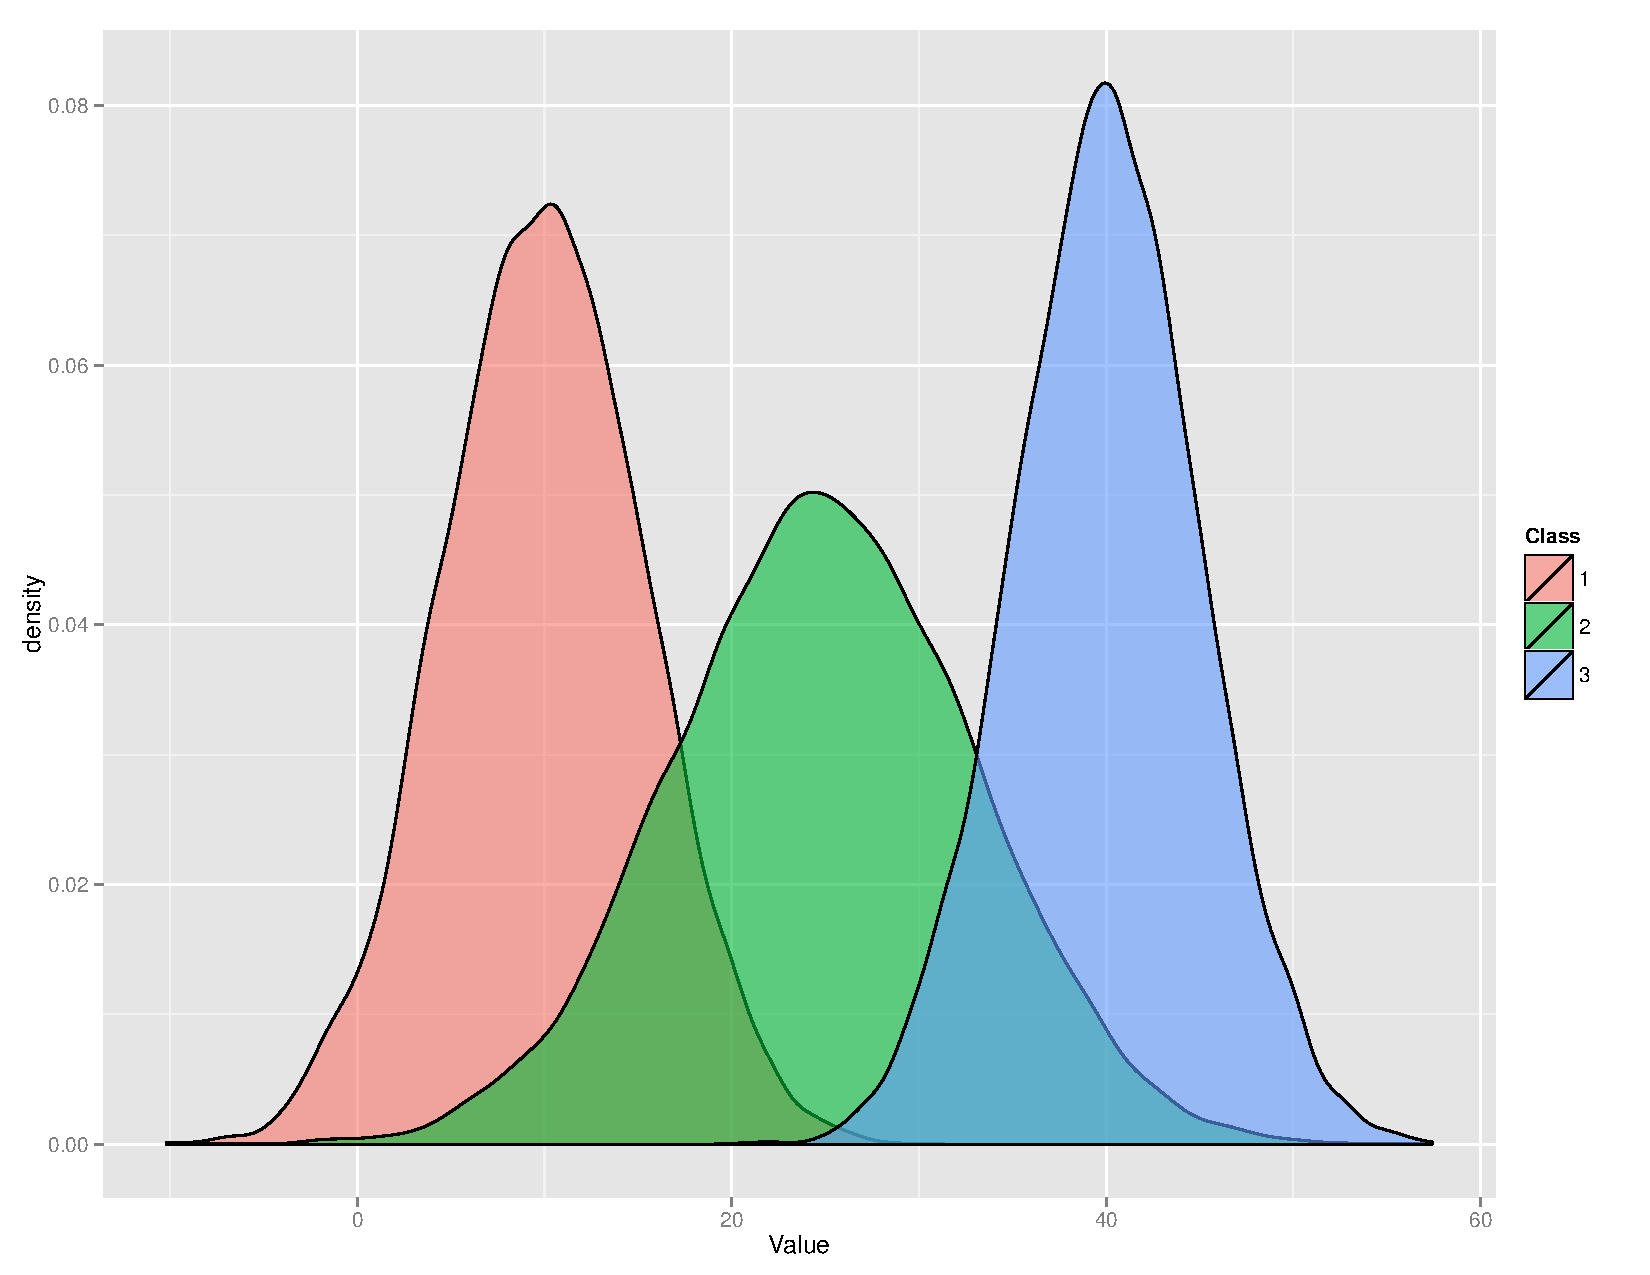
\includegraphics[scale=0.35, trim=0 0 0 0, clip=true] {synthetic-class-distributions.pdf}
\label{fig:indexes}
\end{figure}
\subsubsection{Adults Earnings} 
Taken from the 1994 Census database and hosted on the UCI repository, this dataset represents a real life 50k instance dataset used to predict income levels of adults. This data set is used to see how the system performs in a real world setting but also provides a comparison against other system. The dataset primarily contains discrete features and it's expected label is a binary classification task

\subsubsection{Shuttle Satlog}
This data set, again taken from the UCI repository represents satlog information taken over time. The data contains purely continuous features so gives a foundation for verifying accuracy of the continuous features of the system. Furthermore, the dataset provides a multi class label set to test the performance of the multi-class functionality of the classifier.

\subsection{Load Tests}
As the intension of the system is to not just provide a powerful classifier but also to do so under extreme load within a stream based setting. Consequently a load testing framework called grinder\cite{grinder} is used to apply a distributed load from multiple injector instances onto a single deployment of the RCE system to determine the total amount of throughput it can handle including information on latency and error rates. The implementation is provided in the \verb|performance-test| module.

\chapter{Performance}
\section{Classification Performance}
The following section presents the results of both the performance and load tests as described in the previous chapter.
\clearpage
\subsection{Synthetic Test}
To begin with, the synthetic test is used to evaluate a comparison of the discrete\footnote{The actual synthetic feature values are continuous in nature being drawn from means of the range of 0-300 with similar covariances. Discretization of the feature values occurs as the events are serialized from the test driver by casting to discrete integer values } and continuous feature handlers at fitting a normal mixture model of 10000 training instances.

\begin{figure}[h!]
\centering
\caption{ROC of continuous and discrete feature handlers using 11000 labelled instances and a 5 fold cross validation. The synthetic dataset consists of 3 classification types and 6 features type with distributed mean and covariances for each classification value. A 30\% probability that a given feature will be picked from a uniform distribution is also included to include an element of noise in the dataset}
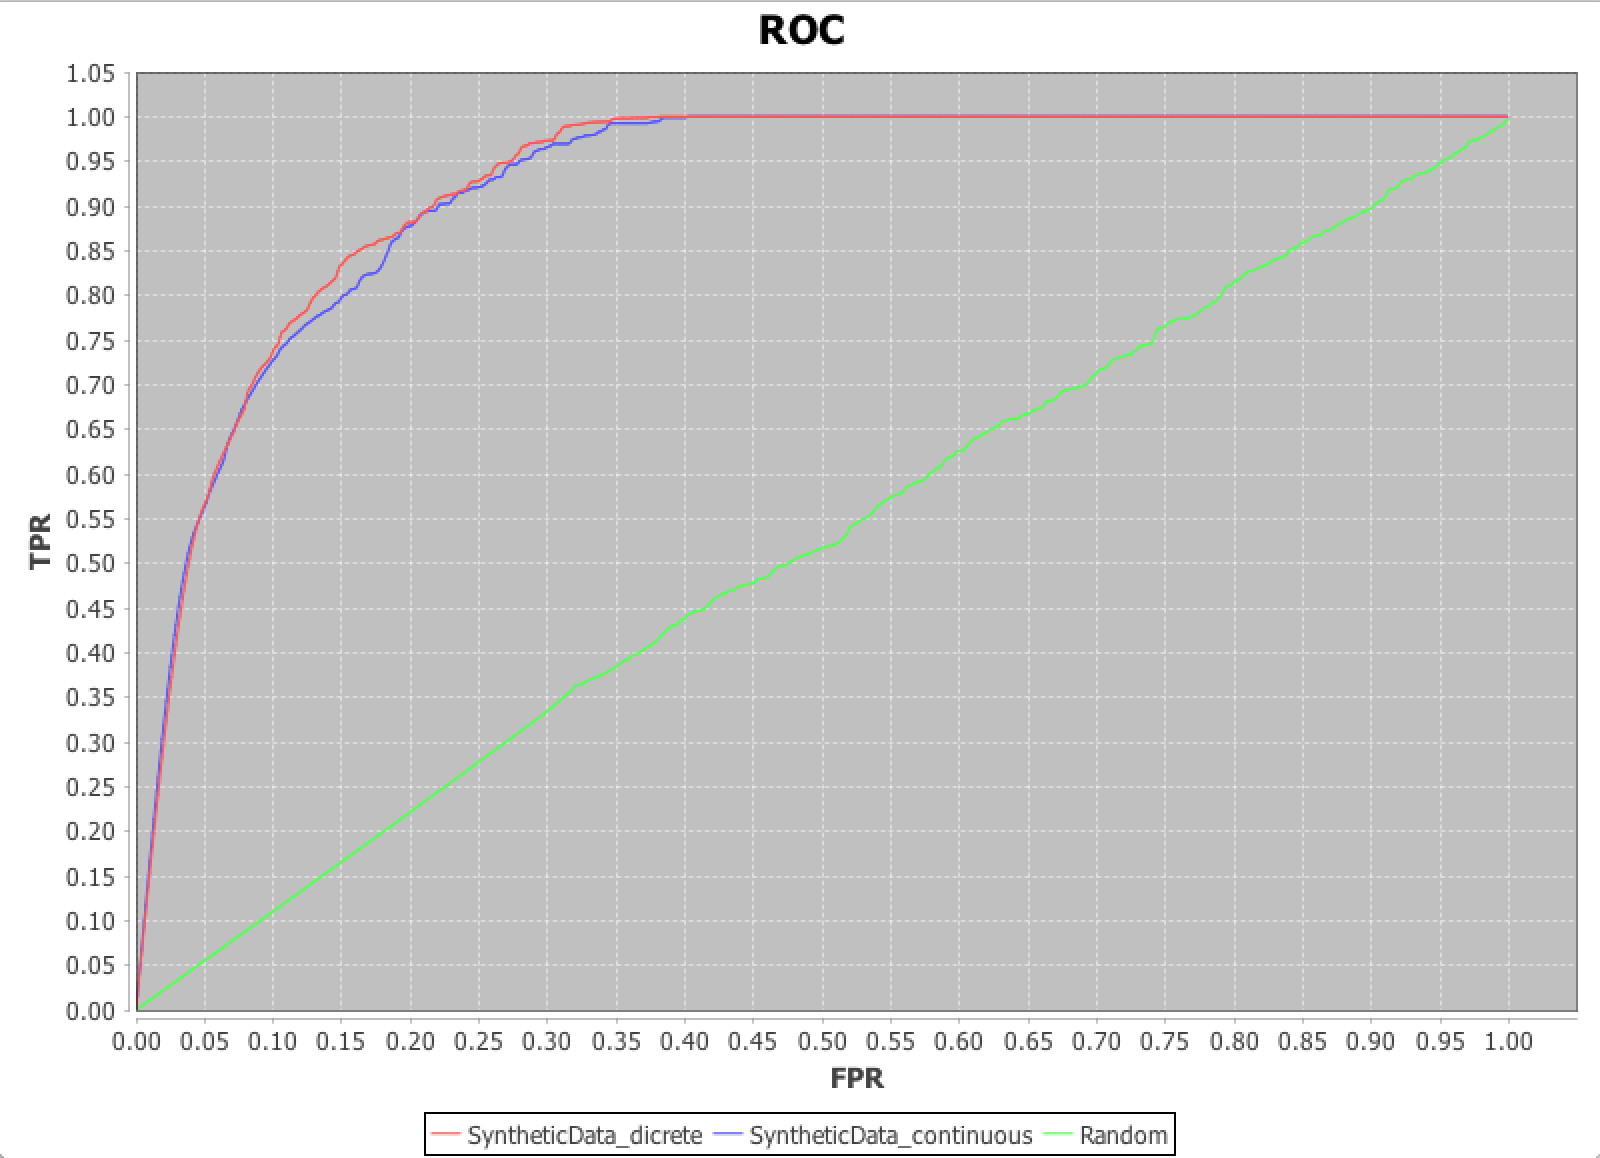
\includegraphics[scale=0.45, trim=0 0 0 0, clip=true] {10000-instance-training-1000-testing-synthetictest.png}
\label{fig:indexes}
\begin{tabular}{l*{60}{c}r}
Test Type & AUC & Accuracy \\
\hline

Synthetic Continuous Feature Handlers & 0.90 & 0.808 \\
Synthetic Discrete Feature Handlers & 0.904 & 0.81 \\

\end{tabular}
\end{figure}

As the discrete and continuous feature handler tests are fairly comparable, another test is performed to see how the two approaches compare in the presence of limited samples\footnote{As the system was built with large scale datasets in mind, such a scenario is not really valid but included for completeness}


\begin{figure}[h!]
\centering
\caption{ROC of continuous and discrete feature handlers using 1100 synthentic instances and 5 fold cross validation}
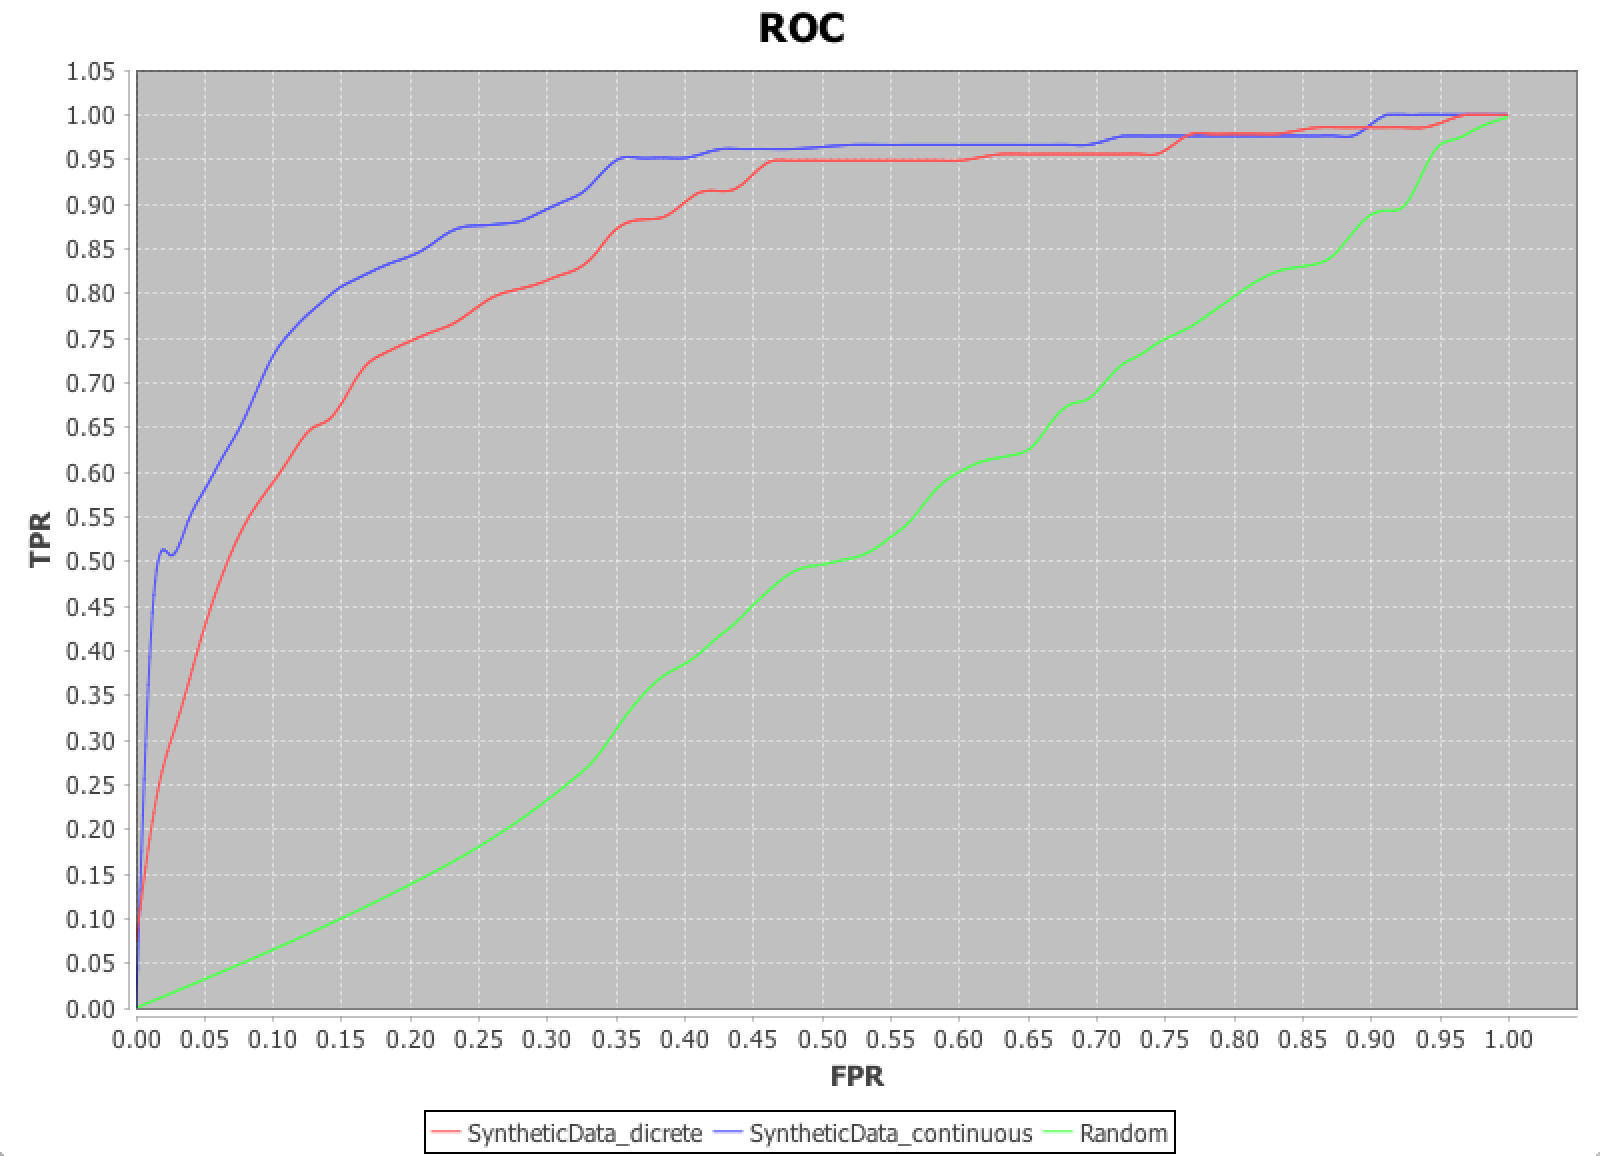
\includegraphics[scale=0.45, trim=0 0 0 0, clip=true] {1000-instance-training-100-testing-synthetictest.png}
\label{fig:indexes}
\begin{tabular}{l*{6}{c}r}
Test Type & AUC & Accuracy \\
\hline
Synthetic Continuous Feature Handlers & 0.872 & 0.8 \\
Synthetic Discrete Feature Handlers & 0.833 & 0.74 \\

\end{tabular}
\end{figure}
\clearpage
\subsection{Adult Wages}
Next the adult wages dataset is considered to offer a comparison of the classifier against other published known implementations. Configuring the system with all features being treated as discrete yields the following ROC curve.
\begin{figure}[h!]
\centering
\caption{ROC of all discrete feature handlers using adult wage test set. N-fold validation is not used in this test so that the provided training/test splits can be used to compare against the published results of different classifiers}
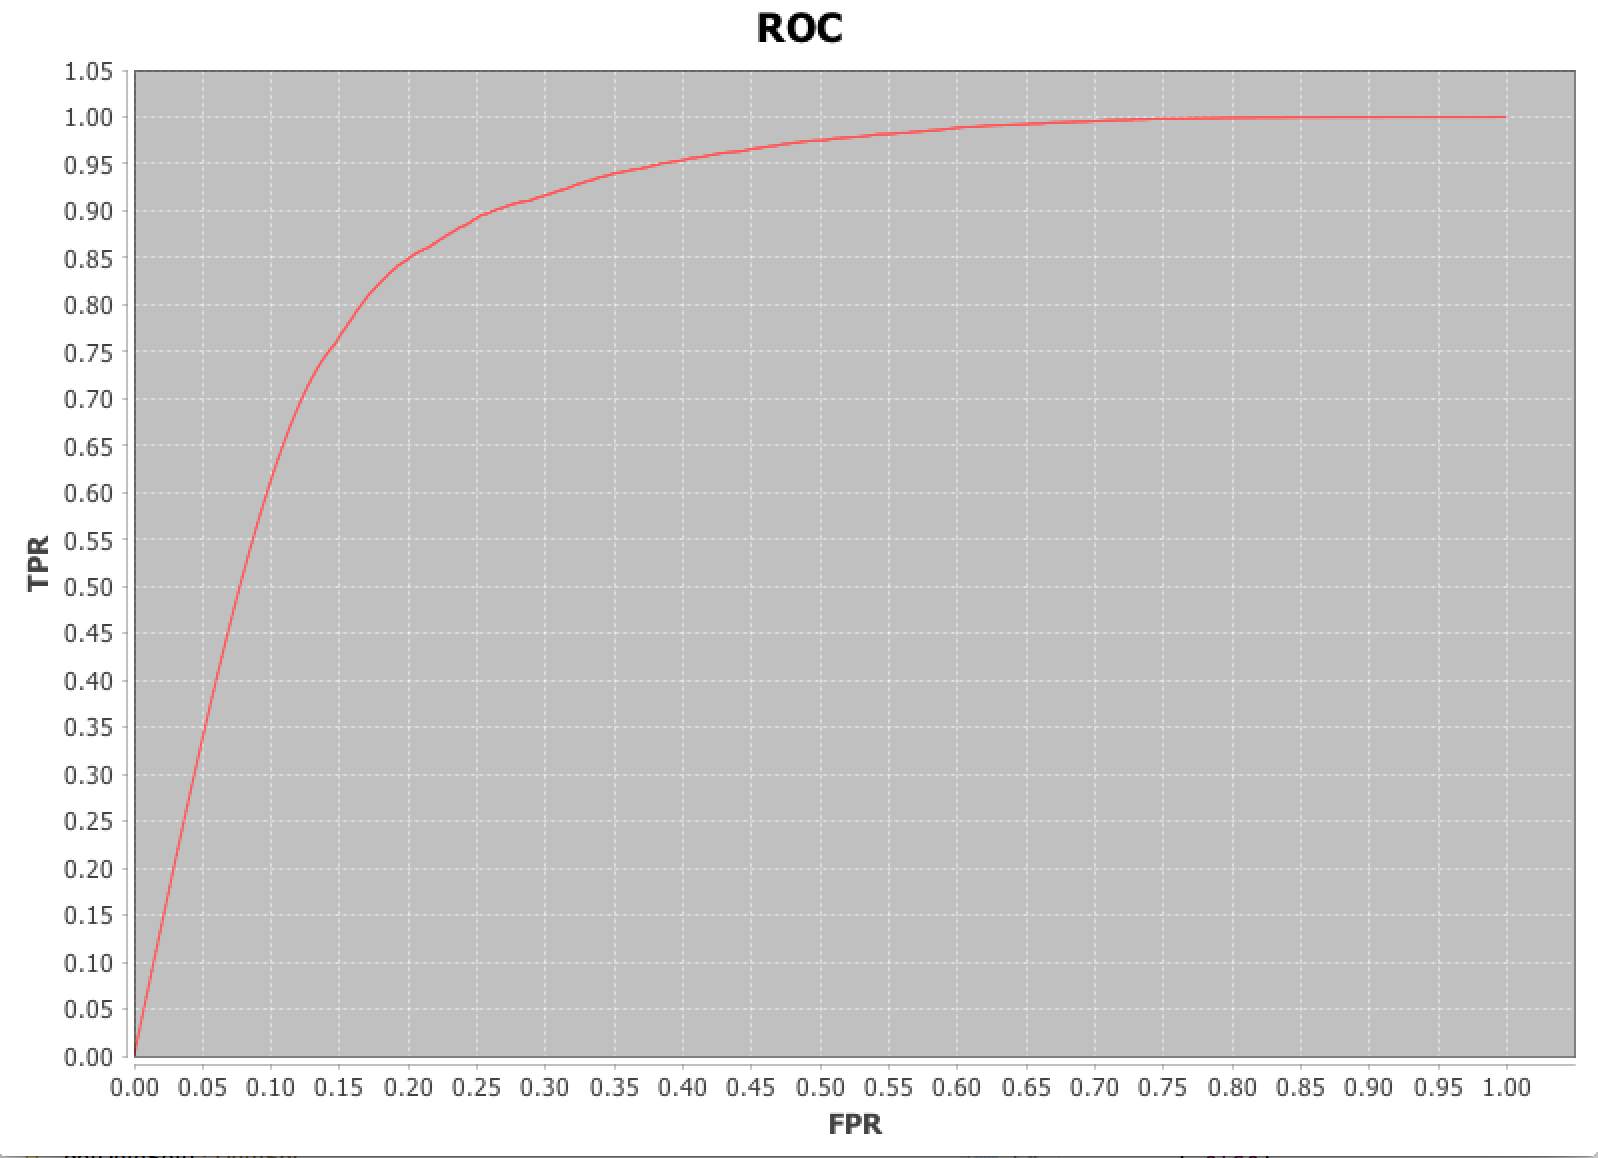
\includegraphics[scale=0.45, trim=0 5 0 0, clip=true] {all_discrete_features_adult_earnings.png}
\label{fig:indexes}
\begin{tabular}{l*{6}{c}r}
Test Type & AUC & Accuracy \\
\hline
Adult Wage Discrete Feature Handlers & 0.858 & 0.837 \\
\end{tabular}
\end{figure}
\\Next a comparison of the performance of the system is considered when different features are considered as being continuous.
\begin{figure}[h!]
\centering
\caption{ROC of using individual feature types configured as continuous features with the rest defined as discrete features. Also includes corresponding model sizes}
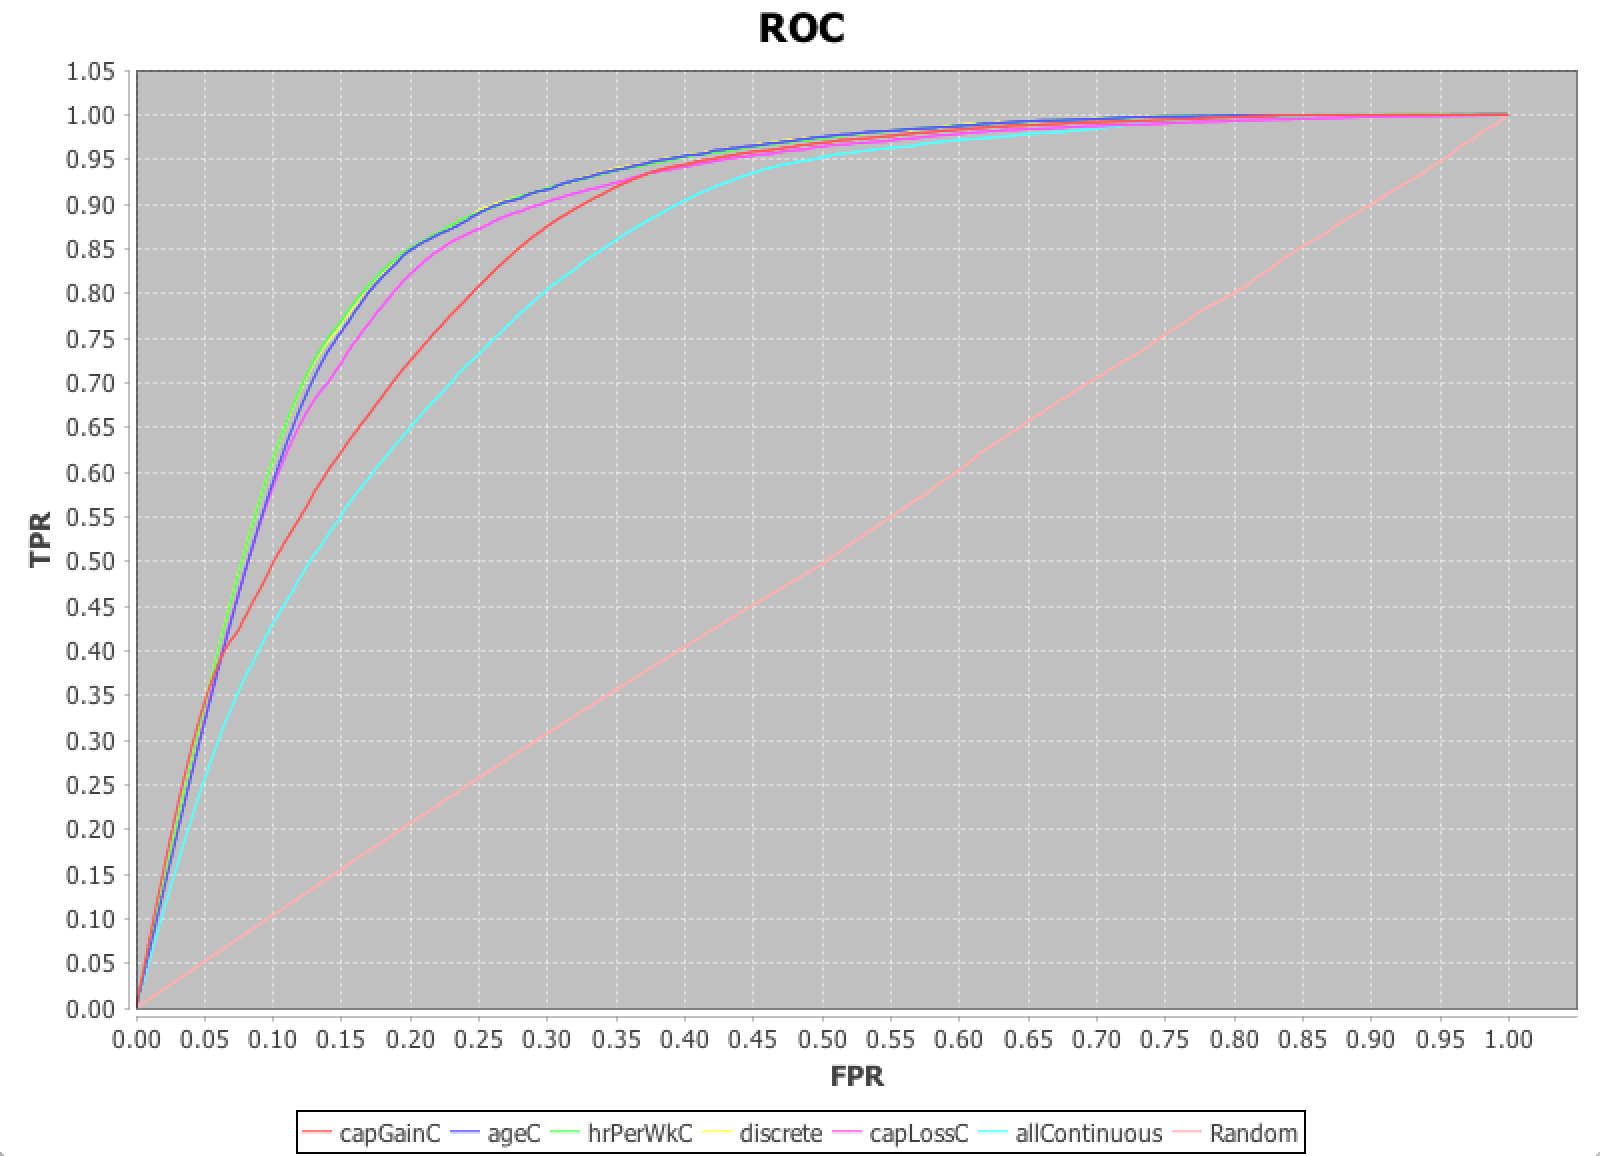
\includegraphics[scale=0.50, trim=0 0 0 2, clip=true] {continuous_features_adult_earnings.png}
\label{fig:indexes}
\begin{tabular}{l*{6}{c}r}
Test Type & AUC & Accuracy & Model Size (bytes)\\
\hline
\verb|capGain| Continuous Feature & 0.800 & 0.849 & 20,345,126 & \\
\verb|age| Continuous Feature & 0.857 & 0.841 & 20,909,350\\
\verb|hrPerWk| Continuous Feature & 0.858 & 0.838 & 20,299,080\\
\verb|capLoss| Continuous Feature & 0.838 & 0.834 & 21,084,010\\
All Continuous Features & 0.767 & 0.829 & 18,360,056\\
All Discrete Features & 0.858 & 0.838 & 24,542,576\\
Random & 0.500 & 0.498 & 1,771,168\footnote{This is the \it{at rest} model size which has seen no actual events}
\end{tabular}
\end{figure}
\clearpage
\subsection{Space Shuttle}
A regression Task
\section{Throughput Performance}
LoadTest results. TCP vs UDP
\chapter{Conclusions}
\section{Results}
Discussion on how the results presented in the performance section compare with other systems.
\section{Limitations}
No FeatureExtraction.
\section{Future Work}
Plugging in more classifiers. Spatial models such as RBF's etc
Static analysis should be conducted,
Bucketed Continuous accumulator types
using object pooling from protostuff rather than Schema.newMessage()

\printbibliography

\end{document}